%%%%%%%%%%%%%%%%%%%%%%%%%%%%%%%%%%%%%%%%%%%%%%%%%%%%%%%%%%%%%%%%%%%%%%%%
\newpage
\section{Sheared and deformed objects}

\subsection{Non-equilibrium static form factor of a reptating chain}
~\\

\begin{figure}[htb]
\begin{center}
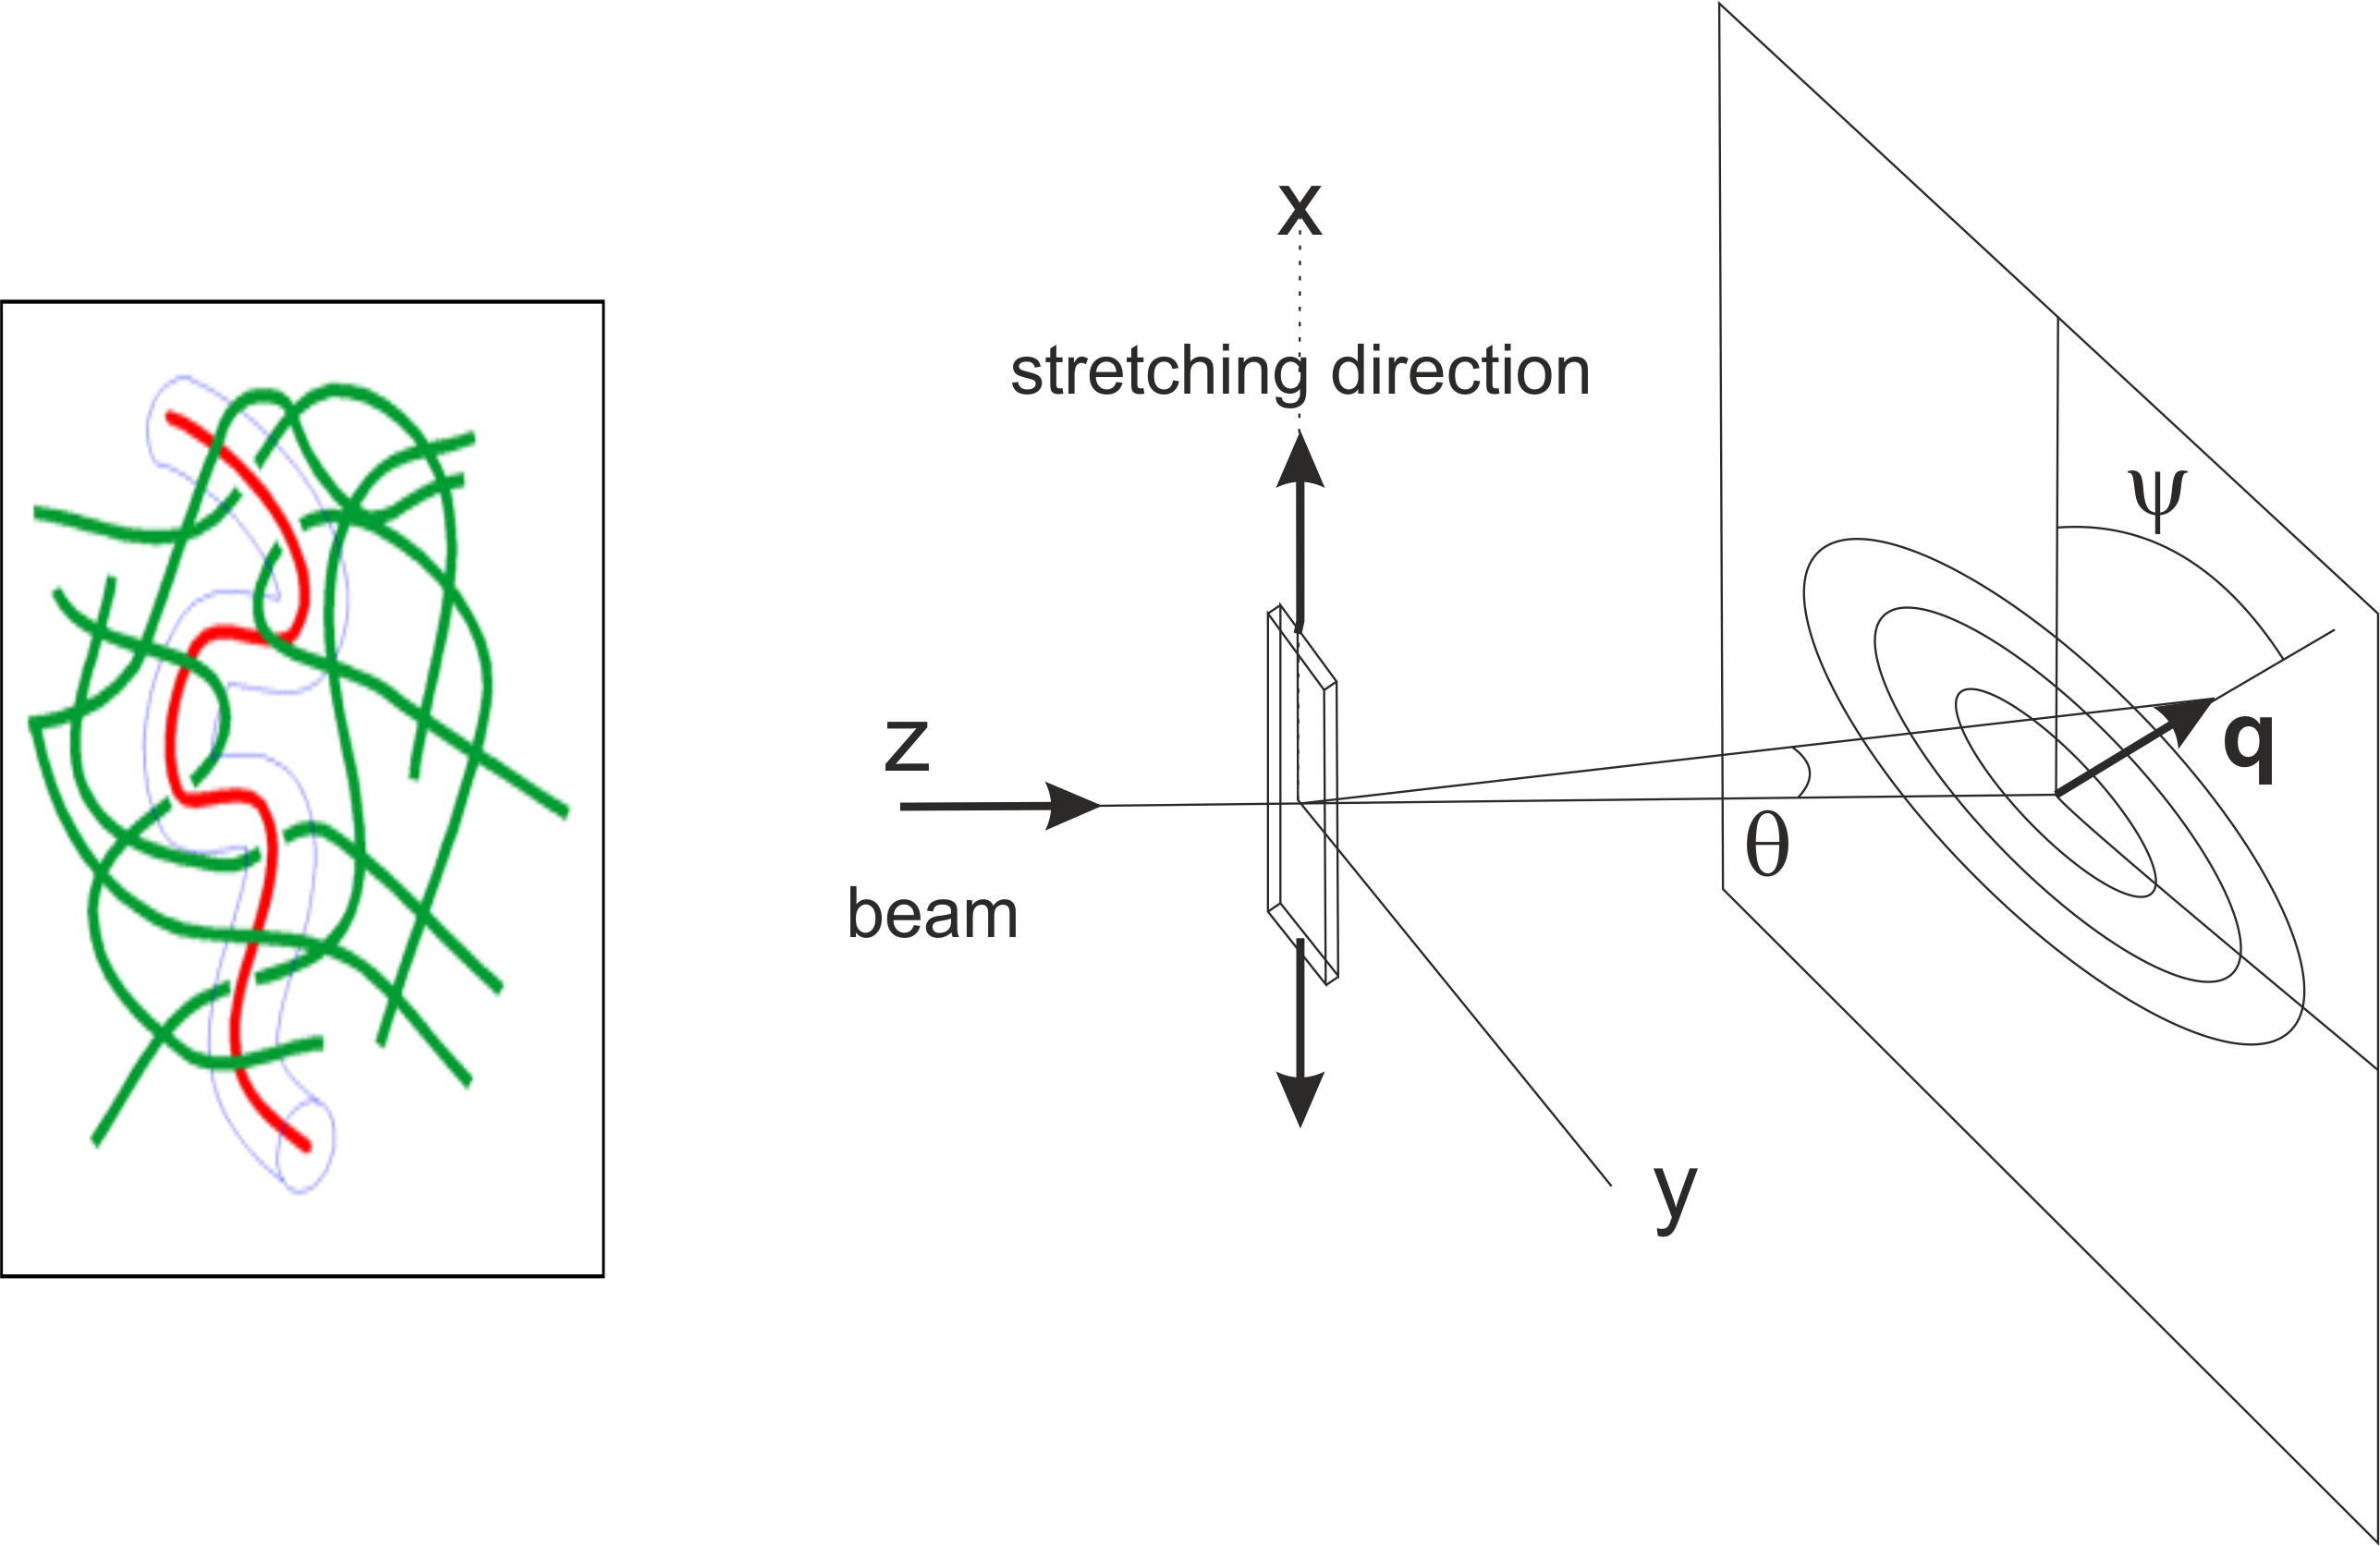
\includegraphics[width=\textwidth]{../images/form_factor/reptating_chain/reptating_chain.png}
\end{center}
\caption{Sketch of experimental setup for stretching a polymer melt.}
\label{fig:stretchpolymermelt}
\end{figure}
This model \cite{Hong1983,Noolandi1984} describes the scattering behaviour of an uniaxial deformed (stretched) Gaussian polymer chain as a function of the deformation ratio and Rouse relaxation time. The model might not include an up-to-date tube model but shows some main features of deformed polymer melts.
\newlength\breites
\settowidth\breites{$\displaystyle {}+{}$}
\begin{align}
\begin{split}
I\left(q,\frac{t}{\tau}\right)/I_0 = & \hspace{\breites}
                                        D(\alpha) + \frac{1}{6}(\alpha-\beta) \left(1+e^{-\alpha}\right) H\left(\alpha,\frac{t}{\tau}\right) \\
                                     & + \frac{1}{6}(\alpha-\beta)^2 e^{-\beta} \int_0^1 \mathrm{d}y \, y^3 e^{\beta y} \left(1+e^{-\alpha y}\right) H\left(\alpha y,\frac{t}{\tau y^2}\right)
\end{split}
\end{align}
with
\begin{align}
H\left(x,\frac{t}{\tau}\right) &= \frac{96}{\pi^2} \sum_{n = \mathrm{odd}} \frac{1}{n^2\left(n^2\pi^2+x^2\right)} e^{-n^2 \frac{t}{\tau}}
\end{align}
$D(x)$ is the Debye function $D(x) = 2\left(x - 1 + e^{-x}\right)/x^2$, $\alpha = q^2 R_g^2$, $R_g$ is the equilibrium radius of gyration
of the chain and $\tau$ is the reptation time or tube disengagement time.
Furthermore $\lambda$ is the uniaxial elongation factor, $q_\parallel$ and $q_\perp$ are respectively the components of the wave vector $q$ in directions parallel and
perpendicular to the direction of elongation which than define the parameter $\beta$ as
\begin{align}
\beta &= \left(q_\parallel^2\lambda^2+q_\perp^2/\lambda\right) R_g^2/E \\
E &= \frac{1}{2} \left\{\lambda +\frac{\mathrm{asinh}\left(\sqrt{\lambda^3-1}\right)}{\sqrt{\lambda\left(\lambda^3-1\right)}} \right\} \\
q_\parallel &= q \cos(\psi-\theta_0) \\
q_\perp &= q \sin(\psi-\theta_0)
\end{align}

\hspace{1pt}\\
\underline{Input Parameters for models \texttt{CylShell1}, \texttt{CylShell2} and \texttt{LongCylShell}:}\\
\begin{description}
\item[\texttt{I0}] forward scattering $I_0$
\item[\texttt{Rg}] radius of gyration of unstretched polymer $R_r$
\item[\texttt{lambda}] stretching factor $\lambda$
\item[\texttt{t/tau}] relaxation time in units of Rouse time $t/\tau$
\item[\texttt{theta\_0}] stretching direction in the detector plane $\theta_0$ in degree
\item[\texttt{psi}] $\mathbf{q}$-direction $\psi$ in the detector plane in degree
\end{description}

\underline{Note:}
\begin{itemize}
\item The model only converges for $\lambda >1$.
\end{itemize}

\begin{figure}[htb]
\begin{center}
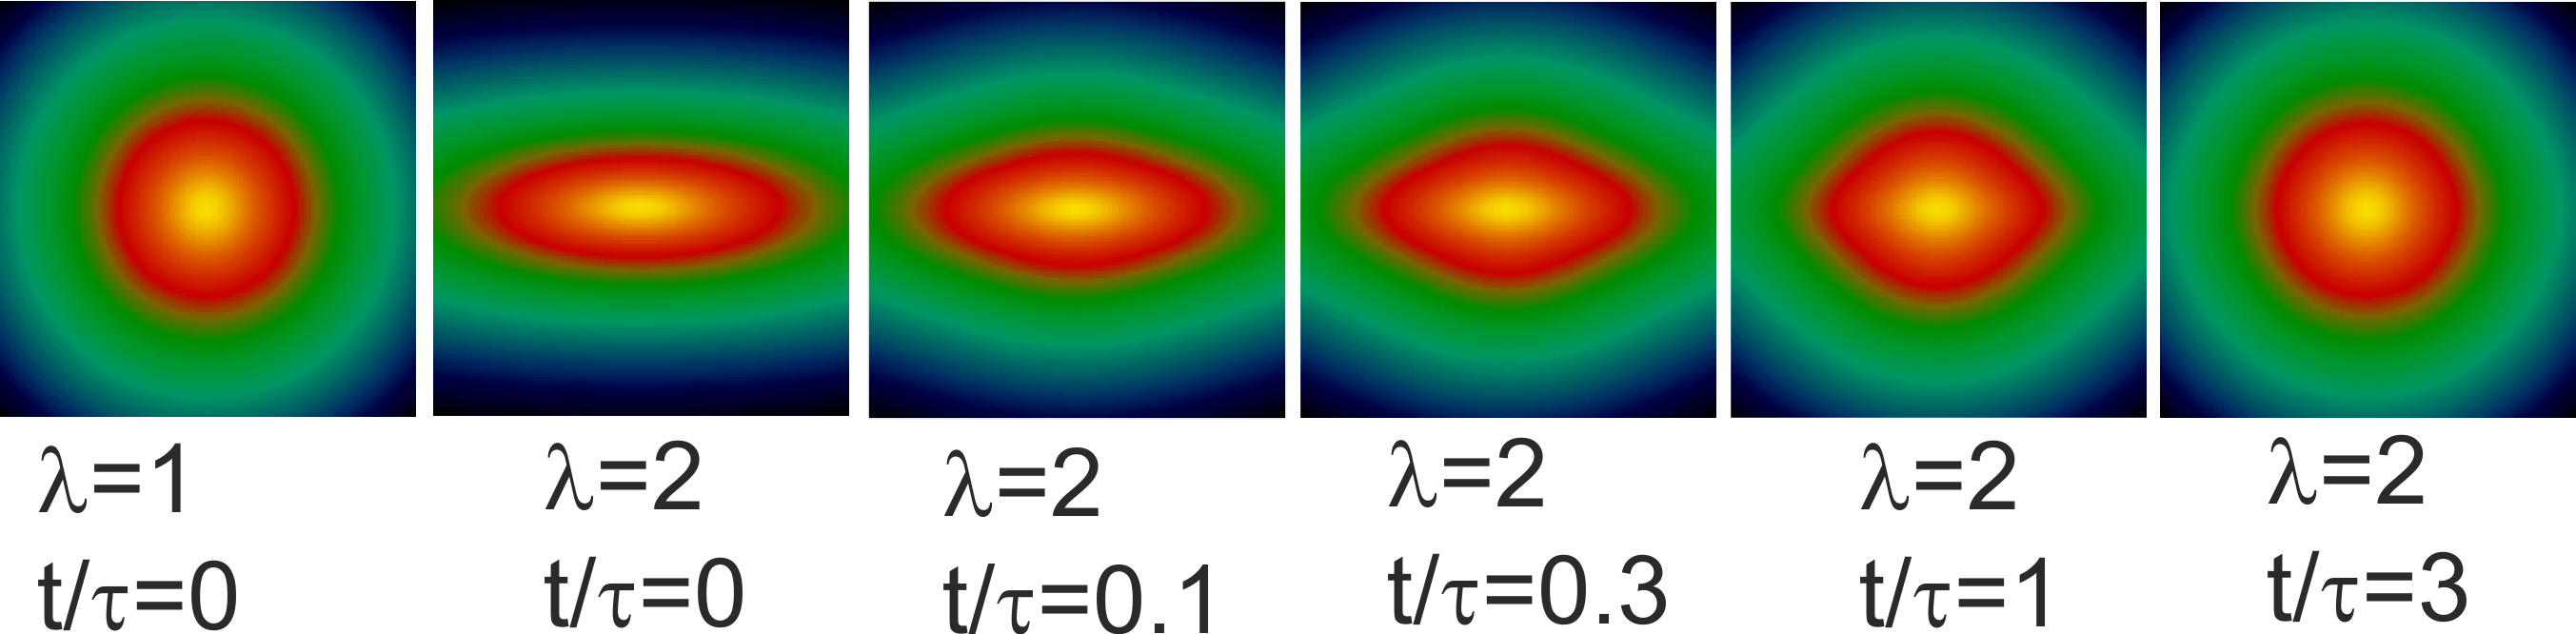
\includegraphics[width=\textwidth]{../images/form_factor/reptating_chain/lambda_2_reptating_chains.png}
\end{center}
\caption{2D scattering patterns for different relaxation times $t/\tau$ after a deformation step of $\lambda=2$}
\label{fig:IQ2Dstretchedpolymermelt}
\end{figure}

%%%%%%%%%%%%%%%%%%%%%%%%%%%%%%%%%%%%%%%%%%%%%%%%%%%%%%%%%%%%%%%%%%%%%%%%%
\newpage
\subsection{Sheared Cylinder according to Hayter and Penfold}
\label{sect:ShearedCylinderHayterPenfold}
\hspace{1pt}\\
The orientation distribution of long cylinders in a shear cell has been studied by \cite{Scheraga1951,Jerrard1959,Hayter1984}. In contrast to the orientation distributions described in the next section this distribution also describes the tilting of the most probable orientation against the flow direction.
\begin{figure}[htb]
\begin{center}
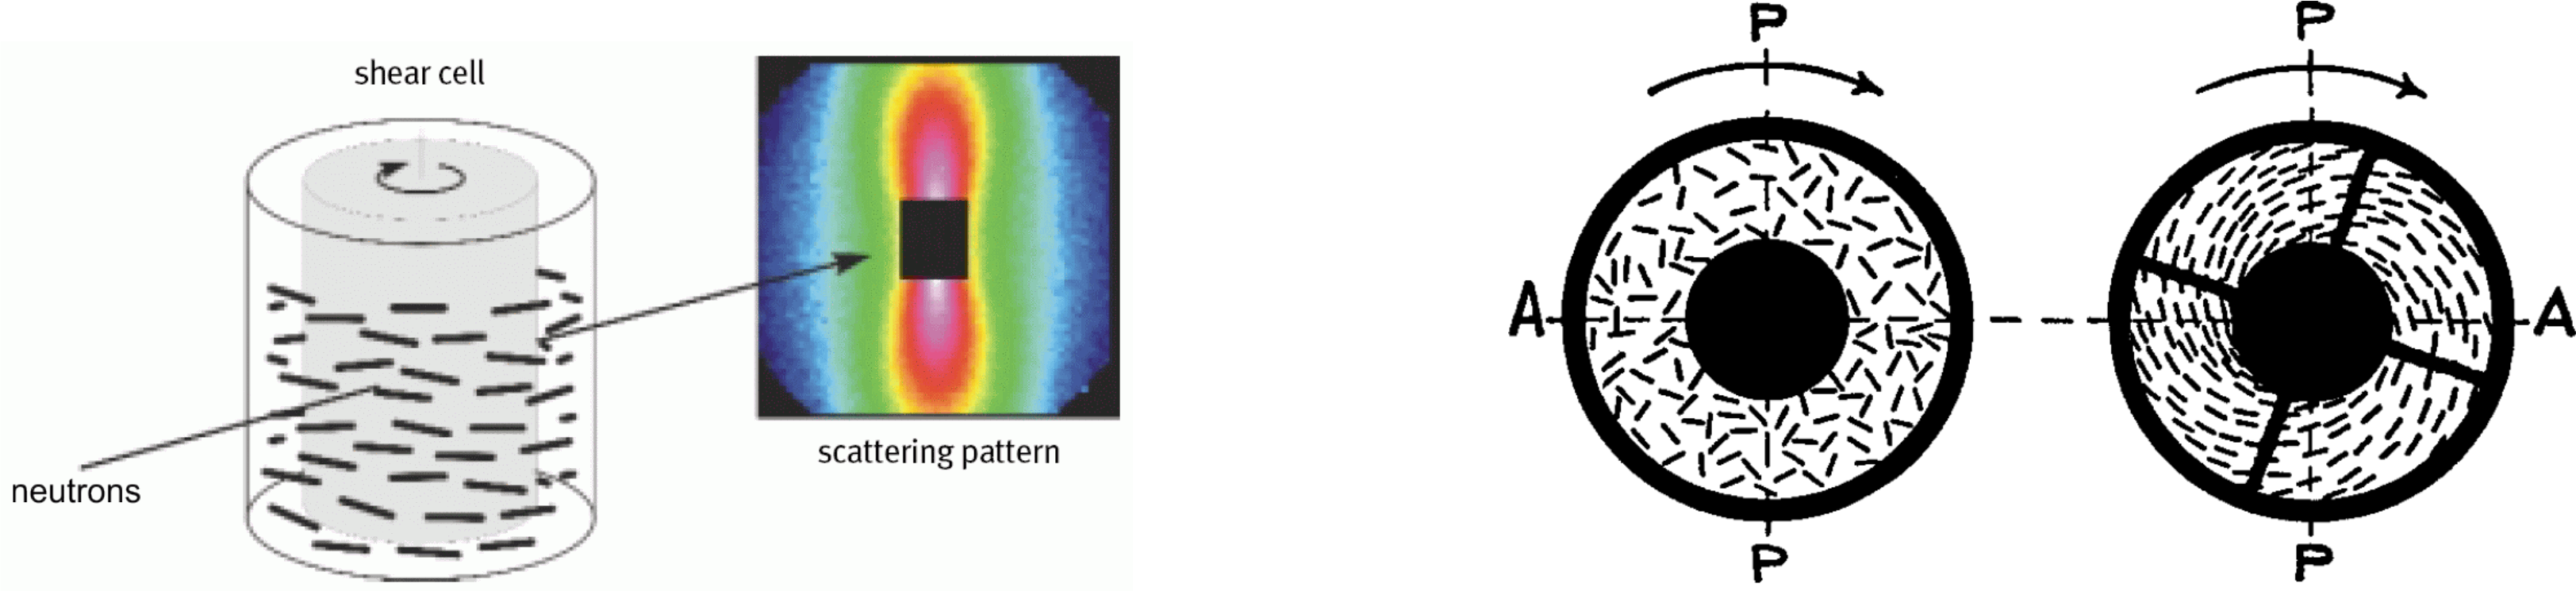
\includegraphics[width=\textwidth]{sheared_cylinders_n_phi0.png}
\end{center}
\caption{Shear orientation of micelles in a shear cell with the
corresponding SANS-pattern. The orientation of rods at rest and under shear according to \cite{Scheraga1951} are shown on th e right as a top view on the cuette cell.} \label{sheared_cylinders1}
\end{figure}

\begin{figure}[htb]
\begin{center}
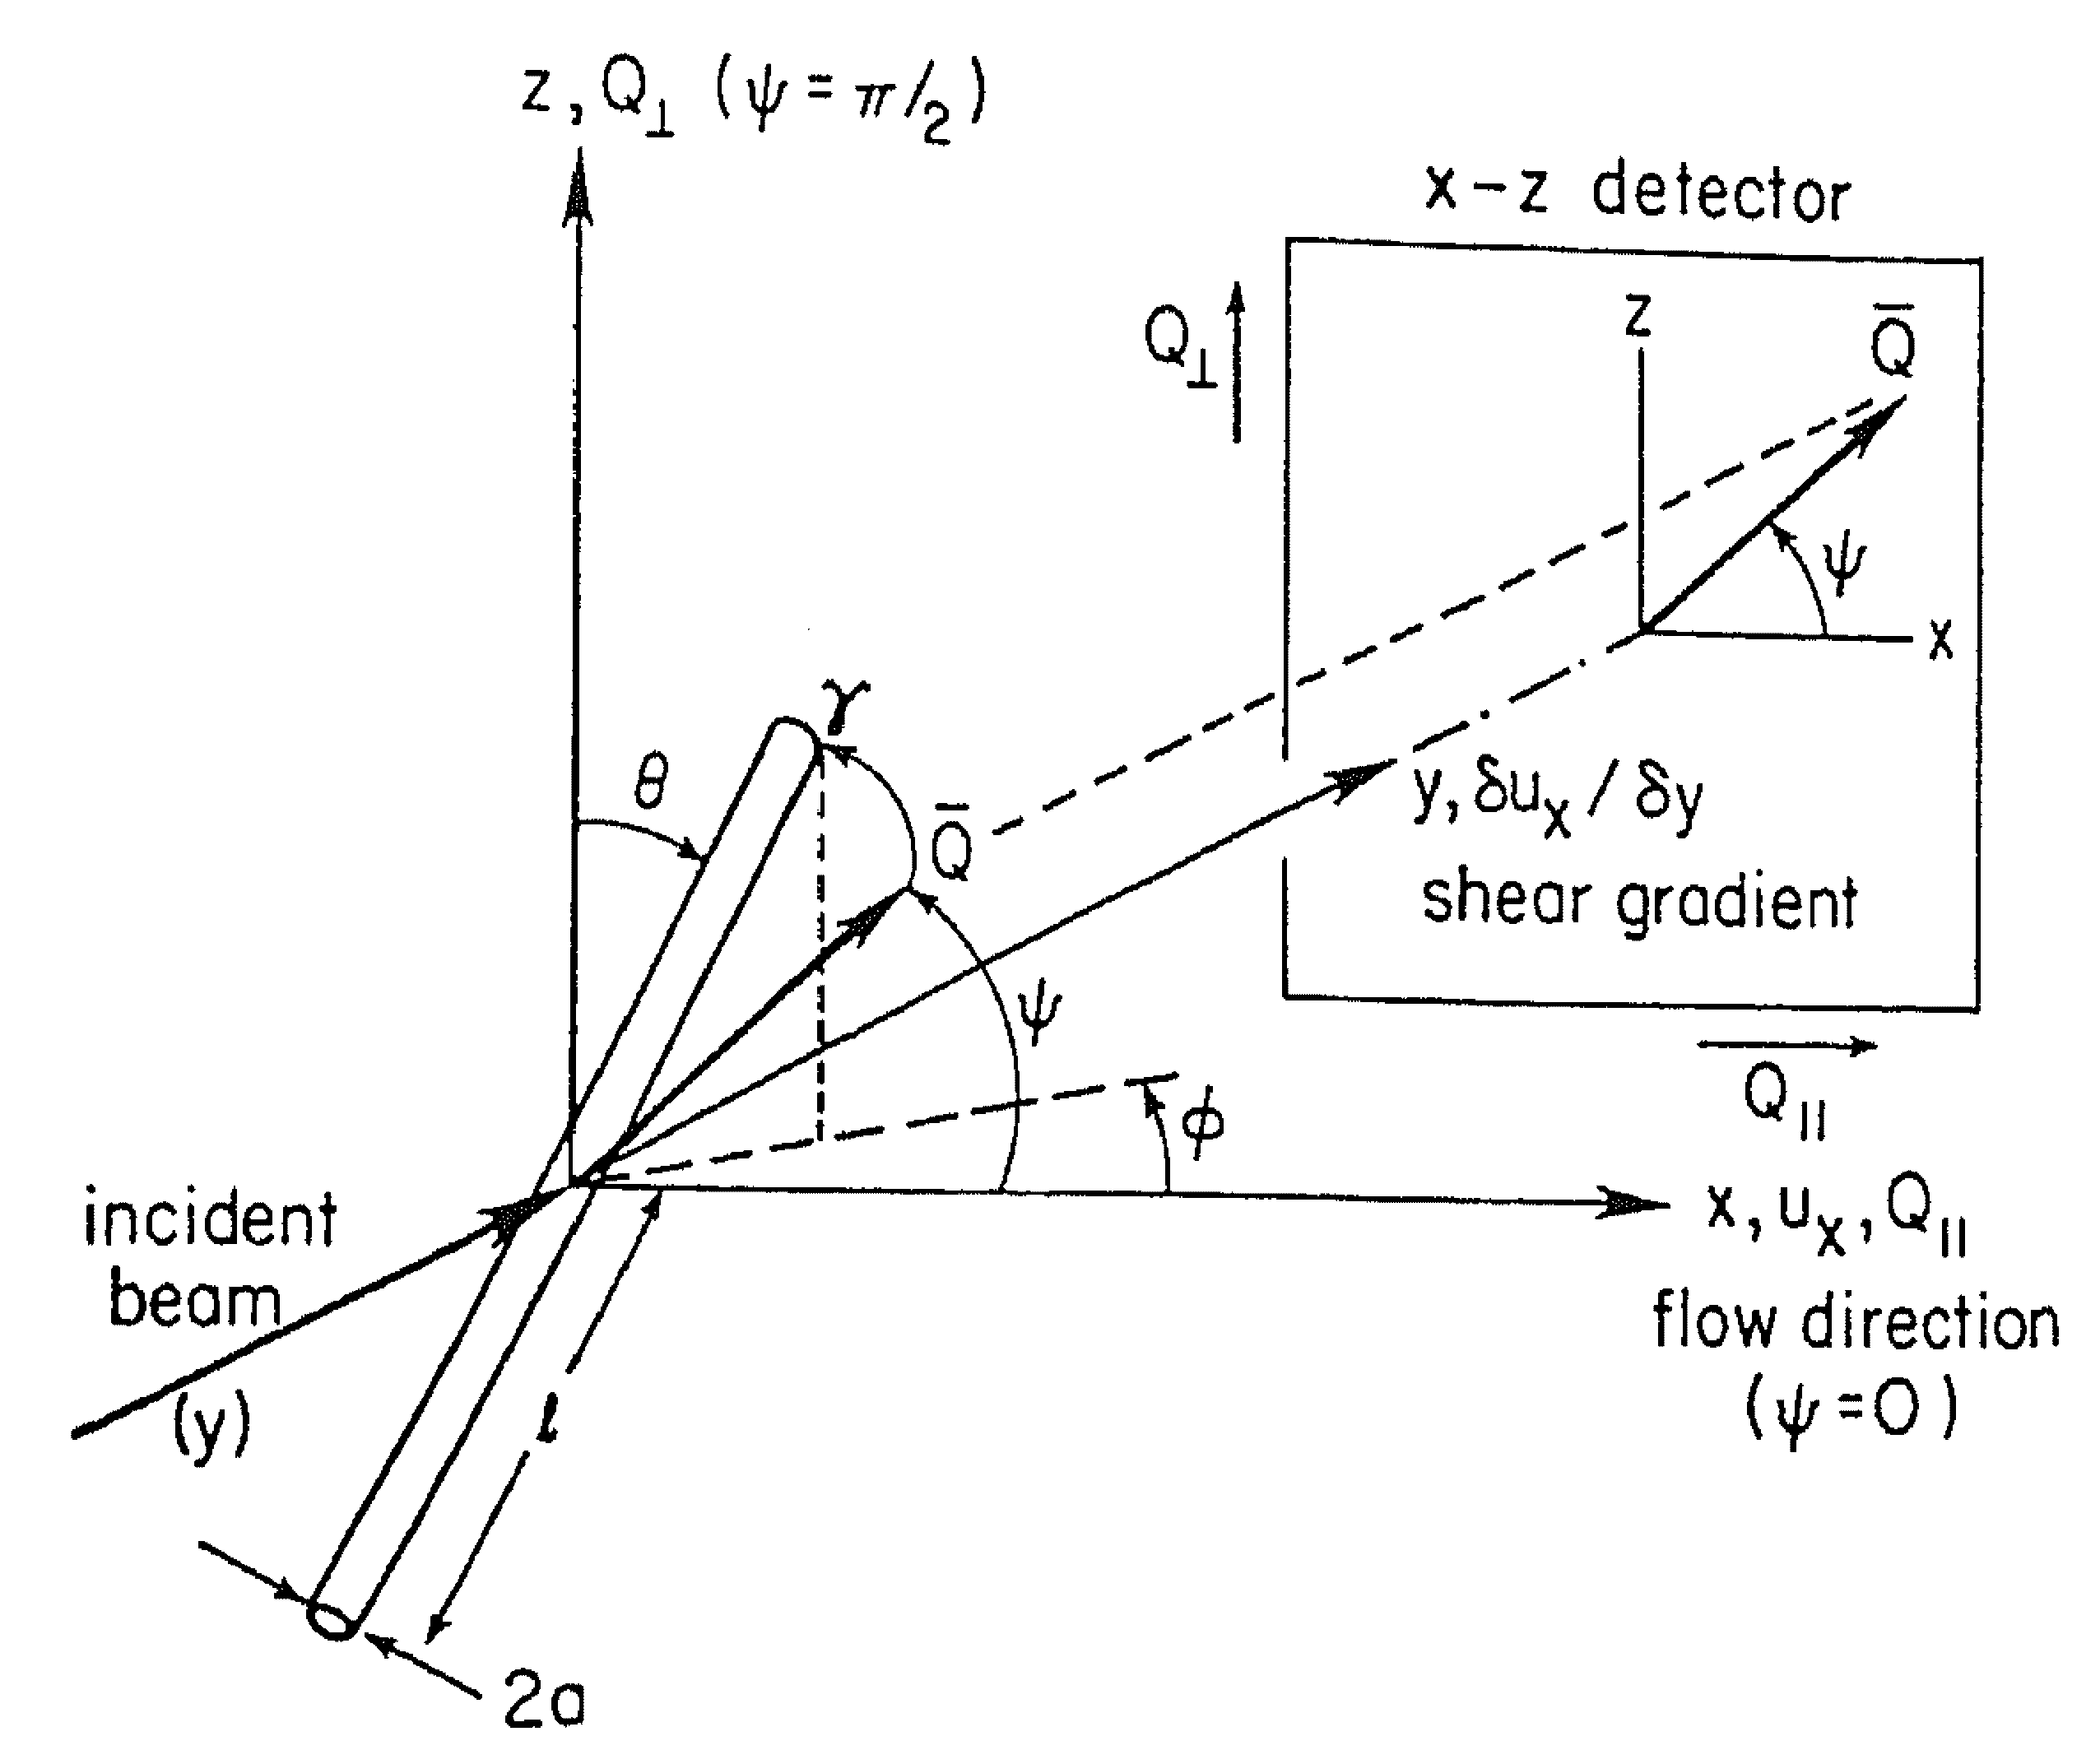
\includegraphics[width=0.7\textwidth]{shear_cuette_SANS_geometry.png}
\end{center}
\caption{Cartesian and angular coordinates referred to the center
of a cylindrical micelle at origin \cite{Hayter1984}. The relationship to the
spectrometer geometry is shown schematically. The momentum
transfer, $Q$, lies in the $z-x$ plane.}
\label{shear_cuette_SANS_geometry}
\end{figure}

The scattering from monodisperse dilute (non-interacting)
isotropic solution of anisotropic micelles is given by \cite{Hayter1984}
\BE
I(Q) =
\left< \vert K_\text{CylSh}(Q)\vert^2 \right>_Q \label{IQ_av}
\EE
where $K(Q)$
is the form factor for a micelle at a given orientation relative
to the momentum transfer $Q$ and $\left<\right>_Q$ denotes an
average over all such orientations.


For a cylindrical shell of length $L$, core diameter $2R$, and shell thickness $t$ the form
factor is given by:
\begin{align}
\begin{split}
K_\text{CylSh}\left(Q,\dots,\gamma\right)  = &
                  \hspace{\breites} K_\text{Cyl}\left(Q,\eta_\text{core}-\eta_\text{shell},R,L,\gamma\right) \\
                               & +  K_\text{Cyl}\left(Q,\eta_\text{shell}-\eta_\text{solv},R+\Delta R,L,\gamma\right)
\end{split}
\end{align}
with
\begin{align}
K_\text{Cyl}(Q,\Delta\eta,R,L,\gamma) & = 2 \pi R^2 L \Delta \eta
    \frac{J_1\left(Q R \sin\gamma\right)}{Q R \sin\gamma} \,
    \frac{\sin\left(\frac{QL}{2} \cos\gamma\right)}{\frac{QL}{2} \cos\gamma}
\end{align}
where $\gamma$ is the angle between $\mathbf{Q}$ and the cylinder
axis $\mathbf{n}$. $\eta_\text{core}$, $\eta_\text{shell}$, and $\eta_\text{solv}$ are the scattering length densities of the cylinder core, shell and solvent. $J_1(x)$ is the first order Bessel function of
the first kind. $\gamma$ can be calculated from the orientation
($\theta$, $\phi$) of the cylinder and the direction of the
scattering vector $\psi$ in the plane of the detector by
where $\gamma$ is the angle between $Q$ and the cylinder axis.

The scattering geometry for shear alignment is shown in Fig.
\ref{shear_cuette_SANS_geometry}. In general perfect alignment
will not be achieved, and an orientation distribution must be
employed such that the resultant scattering will be given by
\begin{align}
I(Q,\psi) &= \int_0^{2\pi} \int_0^\pi
p_\mathrm{HP}(\theta,\phi;\kappa)\, \left(K^2_\text{CylSh}(Q,\gamma^+)+K^2_\text{CylSh}(Q,\gamma^-)
\right) \sin\theta \mathrm{d}\theta \mathrm{d}\phi
\label{eq:IQShear_pHP}
\end{align}
with
\begin{align}
p_\mathrm{HP}(\theta,\phi;\kappa) & = \frac{(1-\cos
2\varPhi_0)(1+\sin^2\theta\cos 2\varPhi_0)^{3/2}}{4\pi\left[
1-\sin^2\theta\cos 2\varPhi_0\cos 2(\phi-\varPhi_0)\right]^2}
\end{align}
and
\BE
2\varPhi_0 = \arctan(8/\kappa)
\EE
$(\cos \varPhi_0,\sin \varPhi_0,0)^T$
is the direction of the most probable orientation $(\theta=\frac{\pi}{2};\phi=\varPhi_0)$. $\varPhi_0$ varies between $\varPhi_0=\frac{\pi}{4}$ for the isotropic case ($\kappa=0$)  to $\varPhi_0=0$ for perfect alignment ($\kappa\rightarrow \infty$).
\begin{figure}[htb]
\begin{center}
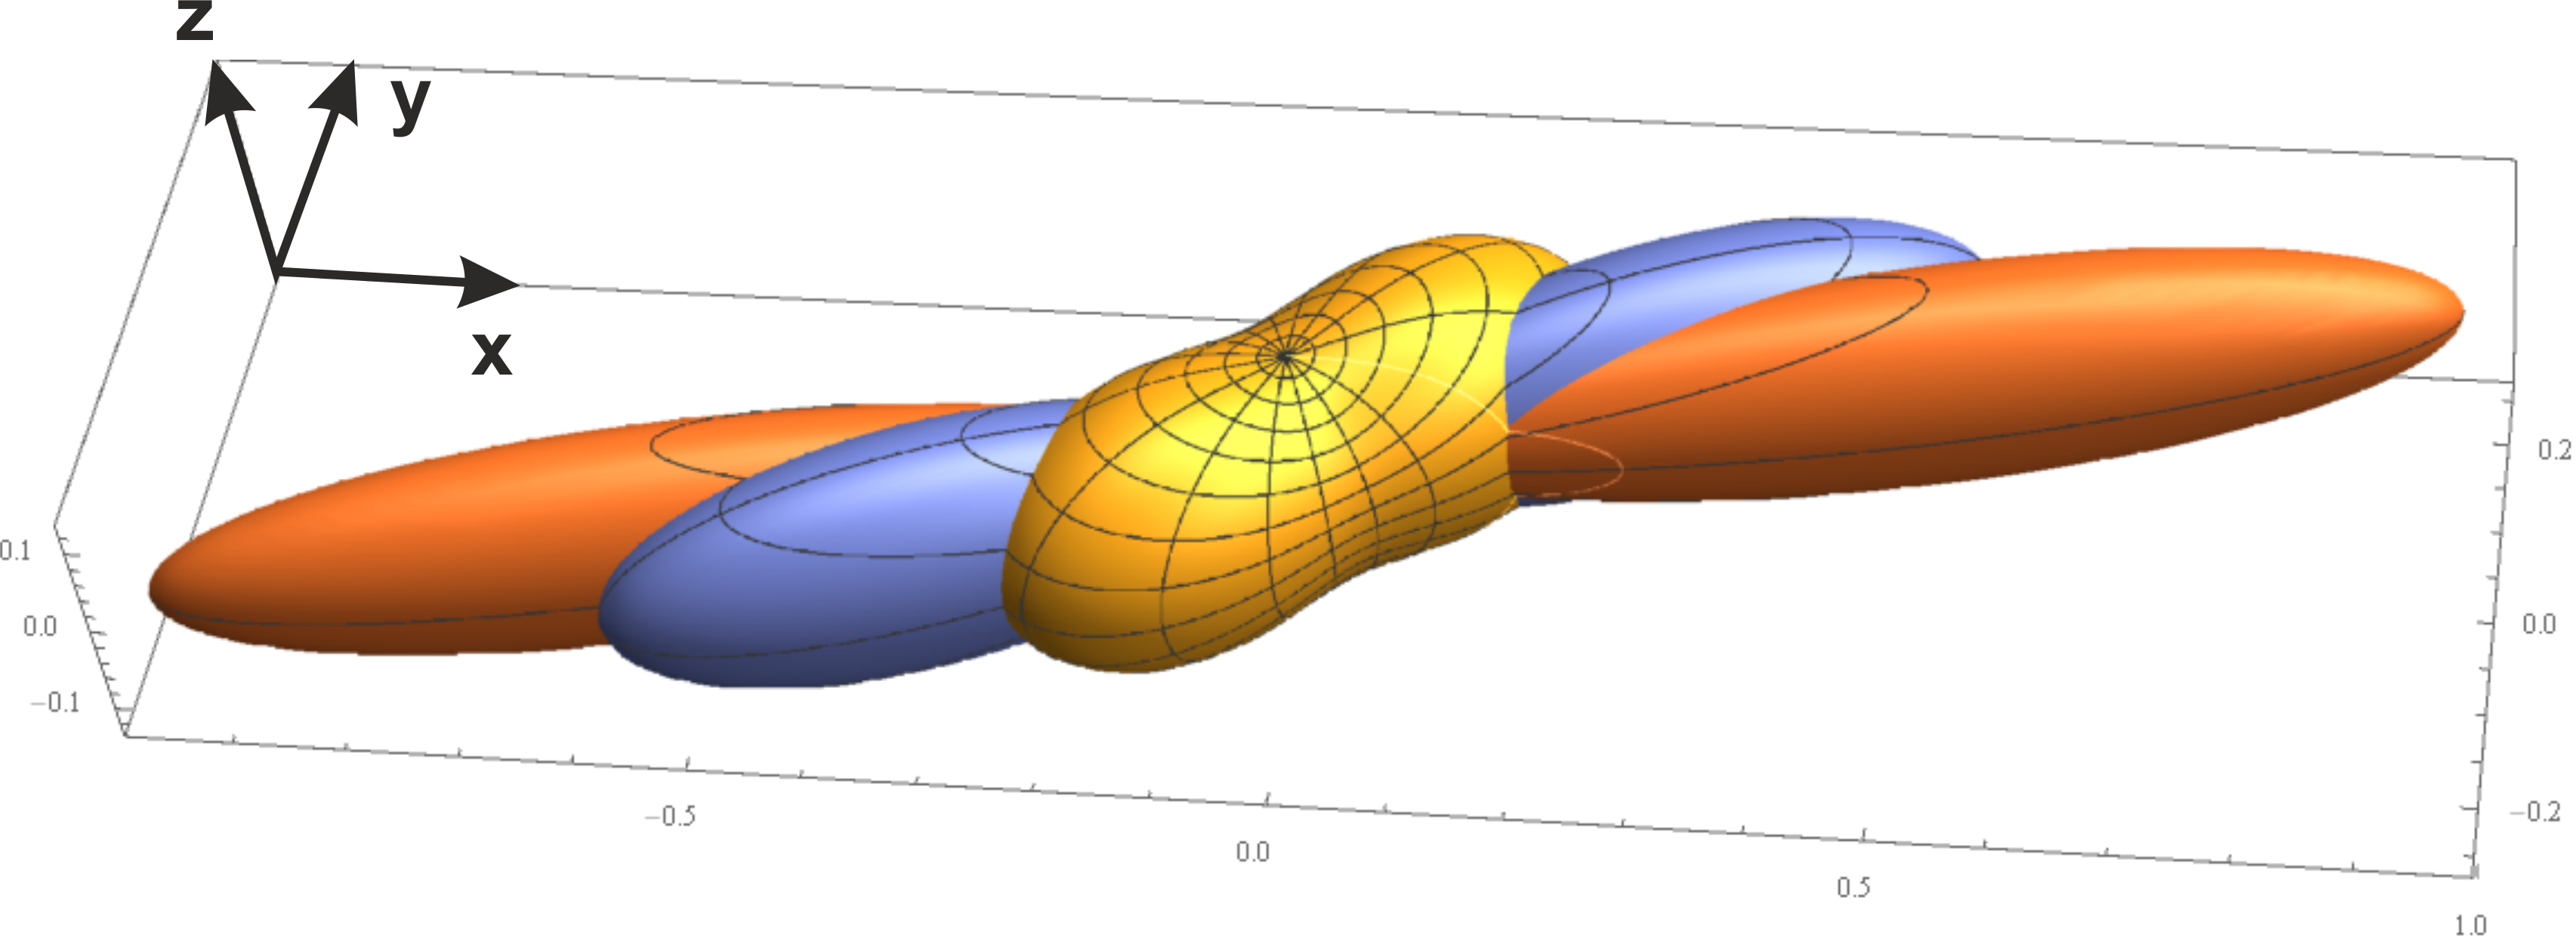
\includegraphics[width=\textwidth]{../images/form_factor/cylindrical_obj/pHP3D.png}
\end{center}
\caption{3D plot of the orientation distributions $2 p_\mathrm{HP}(\theta,\phi;\kappa={2})$ ({\bf \color[rgb]{1.0, 0.85, 0.0}yel-}{\bf \color[rgb]{1.0, 0.85, 0.0}low}), $p_\mathrm{HP}(\theta,\phi;\kappa{=}8)$ ({\bf\color[rgb]{0.36, 0.57, 0.9} blue}), $\frac12 p_\mathrm{HP}(\theta,\phi;\kappa{=}16)$ ({\bf\color[rgb]{1.0, 0.5, 0.0} orange}).} \label{fig:pHP3D}
\end{figure}
As the most probable direction is not the same as the flow direction, which is assumed to be the $x$-direction, and secondly that the beam is passing twice the cuette cell with flow direction $\mathbf{x}$ and $-\mathbf{x}$ we have to take the sum over two values for $\gamma^\pm$ in eq.\ \ref{eq:IQShear_pHP}. The angle $\gamma^\pm = \angle(\mathbf{Q,n}^\pm)$ between the scattering vector $\mathbf{Q}$ and the director of the cylinder axis $\mathbf{n}^\pm$ is
\begin{align}
\frac{\mathbf{Q}}{\abs{\mathbf{Q}}} &=
\begin{pmatrix}
\cos \psi \\
0  \\
\sin \psi
\end{pmatrix} \qquad
\frac{\mathbf{n}^\pm}{\abs{\mathbf{n}^\pm}} =
\begin{pmatrix}
\pm \sin \theta \cos \phi \\
\pm \sin \theta \sin \phi  \\
\cos \theta
\end{pmatrix} \\
\cos \angle(\mathbf{Q,n}^\pm) &= \cos \gamma^\pm = \frac{\mathbf{Q\cdot n}^\pm}{\abs{\mathbf{Q}}\abs{\mathbf{n}^\pm}} =  \pm \cos\psi \sin\theta \cos\phi + \sin\psi \cos\theta
\end{align}
For the reversed direction of the flow the $x$-component of the vector $\mathbf{n}^-$ changes its sign. In the original paper \cite{Hayter1984} one finds $\cos \gamma^-_\mathrm{HP} = \cos\psi \sin\theta \cos\phi - \sin\psi \cos\theta$, which, however, results to the same scattering intensity as the scattering intensity of a cylinder is invariant by a rotation of $\pi$, i.e. as $\cos(\pi+\gamma^-) =-\cos\gamma^- = \cos\gamma^-_\mathrm{HP}$ the resulting scattering patterns are the same for both value $\gamma^-$ and $\gamma^-_\mathrm{HP}$.

\vspace{5mm}

\underline{Input Parameters for model \texttt{Sheared Cylinders (HayterPenfold)}:}\\
\begin{description}
\item[\texttt{R}] radius of cylinders $R$
\item[\texttt{t}] shell thickness $t$
\item[\texttt{L}] cylinder length $L$
\item[\texttt{eta\_core}] scattering length density of cylinder core $\eta_\mathrm{core}$
\item[\texttt{eta\_shell}] scattering length density of cylinder shell $\eta_\mathrm{shell}$
\item[\texttt{eta\_solv}] scattering length density of solvent $\eta_\mathrm{solv}$
\item[\texttt{psi}] direction of scattering vector on the detector $\psi$
\item[{\texttt{sigma}}] width parameter of lognormal size distribution $\sigma$
\item[{\texttt{kappa}}] orientation distribution parameter $\kappa$
\end{description}

\underline{Note:}
\begin{itemize}
\item The size distribution is taken simultaneously over all parameters $R$, $t$ and $L$, so that their aspect rations stay always constant
\item The most probable orientation is not the $\mathbf{x}$-direction but tilted by the angle $\varPhi_0$. As in a rheometer with cuette geometry the beram is passing the sample twice the forward scattering is twice as large as in the model described in the next section.
\item As the orientation distribution is also not rotational symmetric around the direction of the most probably orientation and additional tilted against $\mathbf{x}$-axis the scattering pattern with the order parameter than the orientation distributions look slightly less oriented.
\end{itemize}

%%%%%%%%%%%%%%%%%%%%%%%%%%%%%%%%%%%%%%%%%%%%%%%%%%%%%%%%%%%%%%%%%%%%%%%%%%%%%%%%%%
\newpage
\subsection{partly aligned anisotropic objects}
\label{sect:partlyalignedCylShell}
~\\

In contrast to the model of Hayter and Penfold \cite{Hayter1984} in section \ref{sect:ShearedCylinderHayterPenfold} here we use an orientation distribution with the most probably orientation along the $\mathrm{x}$-axis and independent on the polar angle $\phi$.
Therefore the coordination system is slightly differently defined in the Hayter-Penfold model of sheared cylinders.
\begin{figure}[htb]
\begin{center}
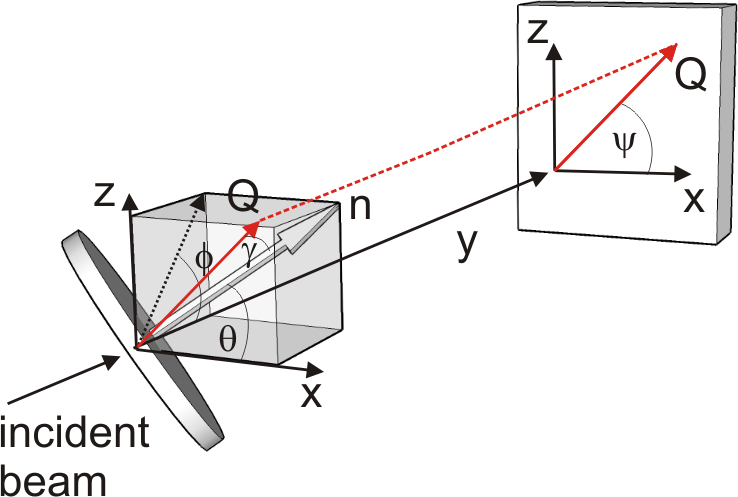
\includegraphics[width=0.7\textwidth]{../images/form_factor/cylindrical_obj/partly_aligned_discs.png}
\end{center}
\caption{Sketch of relative orientation $\mathbf{n}$ of partly
aligned cylinders or discs to the scattering vector $\mathbf{Q}$.}
\label{fig:partly_aligned_discs}
\end{figure}

\noindent The scattering amplitude of a cylindrical shell is given by
\begin{align}
\begin{split}
K_\text{CylShell}\left(Q,\dots,\gamma\right)  = &
\hspace{\breites} K_\text{Cyl}\left(Q,\eta_\text{core}-\eta_\text{shell},R,L,\gamma\right) \\
             & +  K_\text{Cyl}\left(Q,\eta_\text{shell}-\eta_\text{solv},R+\Delta R,L,\gamma\right)
\end{split}
\end{align}
with
\begin{align}
K_\text{Cyl}(Q,\Delta\eta,R,L,\gamma) & = 2 \pi R^2 L \Delta \eta
    \frac{J_1\left(Q R \sin\gamma\right)}{Q R \sin\gamma} \,
    \frac{\sin\left(\frac{QL}{2} \cos\gamma\right)}{\frac{QL}{2} \cos\gamma}
\end{align}
where $\gamma$ is the angle between $\mathbf{Q}$ and the cylinder
axis $\mathbf{n}$. $L$ is the length of the cylinder, $R$ its
radius, $\Delta\eta$ the scattering length density contrast relative
to the solvent and $J_1(x)$ is the first order Bessel function of
the first kind. 

The scattering amplitude of an ellispoid of revolution is given by
\begin{align}
K_\text{Ell}(Q,\Delta\eta,R_\mathrm{e},R_\mathrm{p},\gamma) & = 4\pi R_\mathrm{e}^2 R_{p} \Delta\eta \frac{j_1(Qs)}{Qs}
\end{align}
with $s = \sqrt{R_\mathrm{p}\cos^2\gamma + R_\mathrm{e}\sin^2\gamma}$ and $j_1(x)$ being the spherical bessel function of first kind. $R_\mathrm{e}$ and $R_{p}$ are the equatorial and polar semi-axes of the spheroid, respectively.
The scattering amplitude of an ellipsoidal shell is given by
\begin{align}
\begin{split}
K_\text{EllShell}\left(Q,\dots,\gamma\right)  = &
\hspace{\breites} K_\text{Ell}\left(Q,\eta_\text{core}-\eta_\text{shell},R_{\mathrm{p}},R_{\mathrm{e}},\gamma\right) \\
             & +  K_\text{Ell}\left(Q,\eta_\text{shell}-\eta_\text{solv},R_{\mathrm{p}}+\Delta R,R_{\mathrm{e}}+\Delta R,\gamma\right)
\end{split}
\end{align}
$\gamma$ can be calculated from the orientation
($\theta$, $\phi$) of the cylinder and the direction of the
scattering vector $\psi$ in the plane of the detector by
\begin{align}
\frac{\mathbf{Q}}{\abs{\mathbf{Q}}} &=
\begin{pmatrix}
\cos \psi \\
0  \\
\sin \psi
\end{pmatrix} \qquad
\frac{\mathbf{n}}{\abs{\mathbf{n}}} =
\begin{pmatrix}
\cos \theta \\
\sin \theta \cos \phi  \\
\sin \theta \sin \phi
\end{pmatrix} \\
\cos \measuredangle(\mathbf{Q,n}) &= \cos \gamma = \frac{\mathbf{Q\cdot
n}}{\abs{\mathbf{Q}}\abs{\mathbf{n}}} = \cos\psi \cos\theta +
\sin\psi \sin\theta \sin\phi
\end{align}
If the orientation distribution of the orientation vector $\mathbf{n}$ is described by $p(\theta,\phi,\kappa)$
so that the scattering intensity is given by
\begin{align}
I_\mathrm{p.a.CylShell}(Q) & =
            \int_0^\pi d\theta \int_0^{2\pi} d\phi \, \,
                K^2_\text{CylShell}\left(Q,\dots,\gamma\right)\,p(\theta,\phi;\kappa)\,\sin(\theta) \\
I_\mathrm{p.a.EllShell}(Q) & =
            \int_0^\pi d\theta \int_0^{2\pi} d\phi \, \,
                K^2_\text{EllShell}\left(Q,\dots,\gamma\right)\,p(\theta,\phi;\kappa)\,\sin(\theta)
\end{align}
For this form factor it is assumed that the orientation distribution is independent of $\phi$,
i.e. $p(\theta,\phi;\kappa)=p(\theta;\kappa)$ and that $p(\theta;\kappa)=p(\pi-\theta;\kappa)$, which means that turning the cylinder by 180$^\circ$ results in the same scattering intensity.
Several orientation distributions have been implemented in a way that their resulting order parameter $S_2$ can have values between -0.5 and 1, which correspond to perfect alignment perpendicular to the $\mathrm{x}$ axis and perfect alignment parallel to it. All probability distributions have been normalized 
\begin{align}
\int_0^\pi \int_0^{2\pi} p(\theta,\phi;\kappa) \sin \theta \, d\theta \, d\phi&=1
\end{align}
\begin{figure}[htb]
\begin{center}
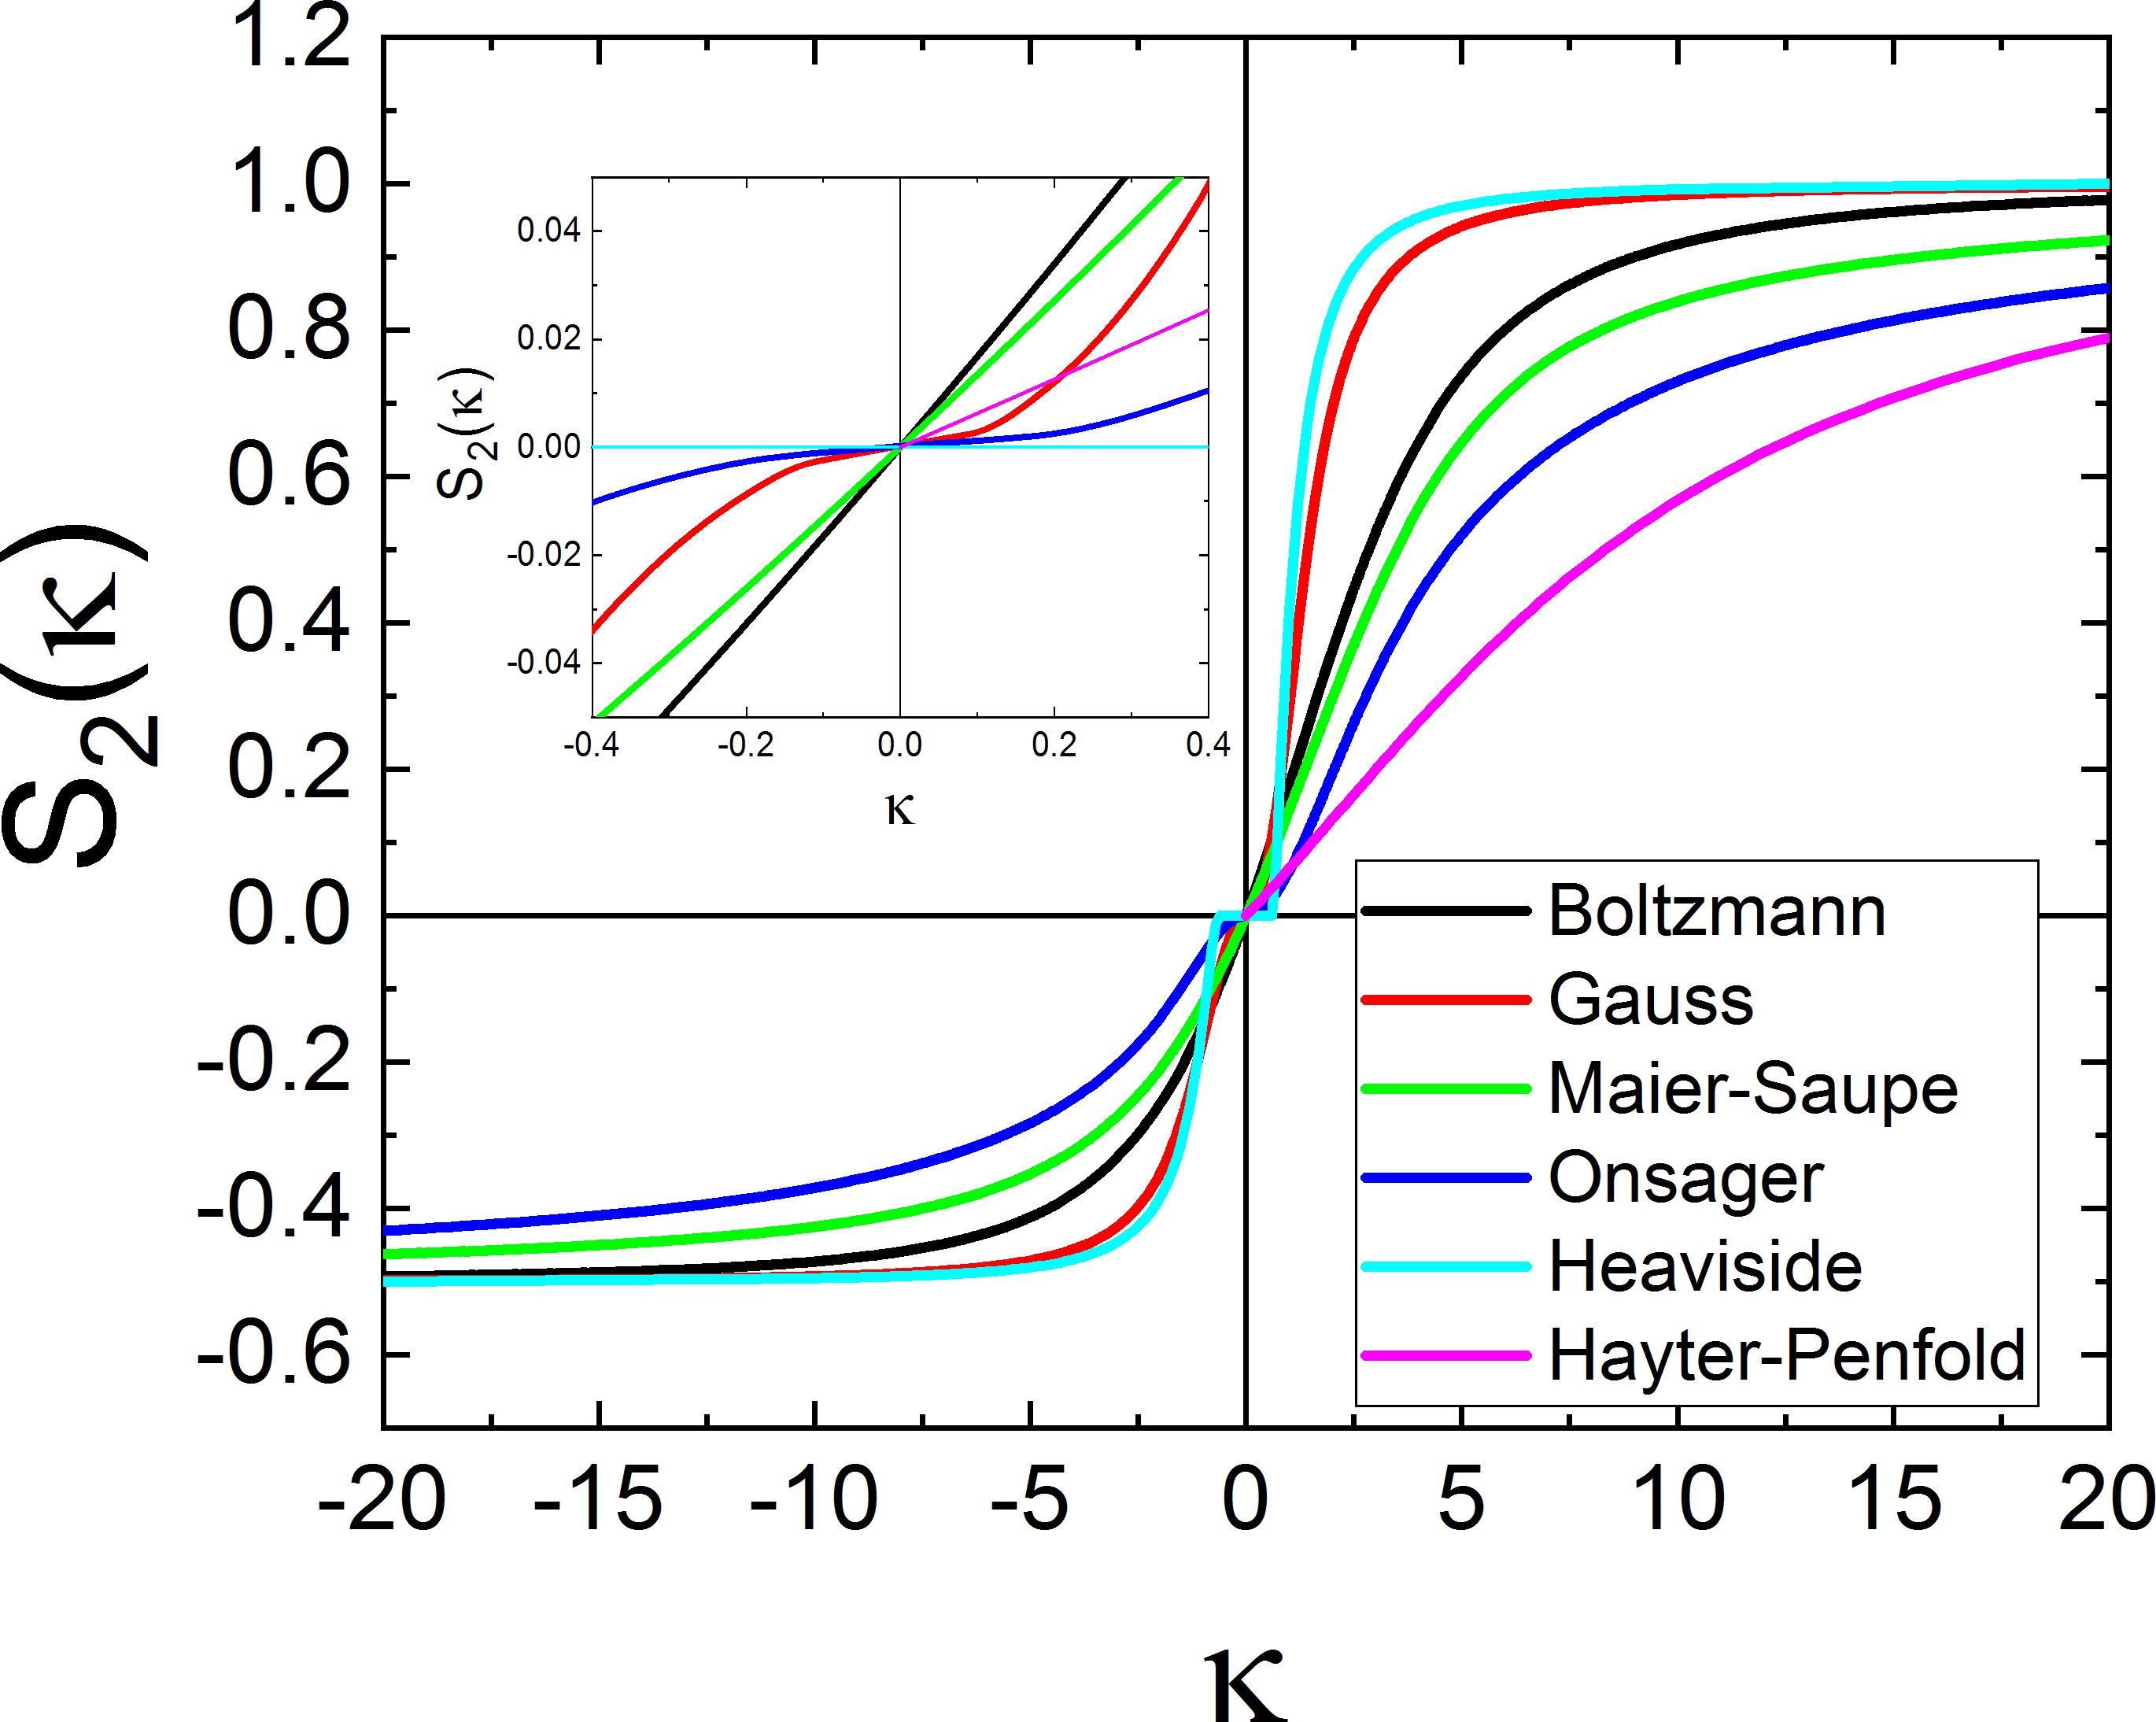
\includegraphics[width=0.75\textwidth]{../images/form_factor/cylindrical_obj/S2(kappa).png}
\end{center}
\caption{Order parameter $S_2(\kappa)$ for the orientation distributions described in the next subsections.}
\label{fig:S2_kappa}
\end{figure}

\begin{table}[htb]
\centering
\caption{Values for $\kappa$ to obtain certain order parameters $S_2(\kappa)$ for the different orientation distributions $p(\theta,\phi,\kappa)$.}
\label{tab:kappas}
\begin{tabular}{|l|llllllllll|}
\toprule
\diagbox{$p(\theta,\phi,\kappa)$}{$S_2(\kappa)$}  & -0.45    & -0.4    & -0.2    & 0 & 0.2    & 0.4    & 0.6    & 0.8    & 0.9    & 0.95    \\ \midrule
Gauss       & -3.739 & -1.62  & -1.128 & 0 & 0.83  & 1.220 & 1.686 & 2.576 & 3.762 & 5.4    \\
Boltzmann   & -7.141 & -4.59  & -1.431 & 0 & 1.114 & 2.218 & 3.581 & 5.989 & 9     & 13.08 \\
Maier-Saupe & -15    & -7.49  & -1.874 & 0 & 1.367 & 2.709 & 4.444 & 8.241 & 15.59 & 30.54 \\
Onsager     & -28.43 & -13.35 & -2.918 & 0 & 2.042 & 3.629 & 6.313 & 13.92 & 28.96 & 58.99 \\
Heavyside   & -3.108 & -2.157 &	-1.129 & 0 & 0.794 & 0.982 & 1.267 & 1.868 & 2.692 & 3.840 \\
Hayter-Penfold   & $\varnothing$ & $\varnothing$&	$\varnothing$ & 0 & 3.008 & 6.269 & 10.93 & 20.8 & 34.91 & 55.64  \\ \bottomrule
\end{tabular}
\end{table}

The order parameters $S_2$ can be calculated by
\begin{align}
S_2(\kappa) &=
\int_0^\pi \int_0^{2\pi}
                p(\theta,\phi;\kappa) \frac12 \left(3\cos^2\theta - 1\right) \sin \theta \, \mathrm{d}\theta\, \mathrm{d}\phi \nonumber \\
&= \int_0^\pi 2\pi
                p(\theta;\kappa) \frac12 \left(3\cos^2\theta - 1\right) \sin \theta \, \mathrm{d}\theta
\label{eq:S2kappa}
\end{align}
\begin{figure}[htb]
\subfigure[Onsager orientation distribution for $\kappa=3$. ]{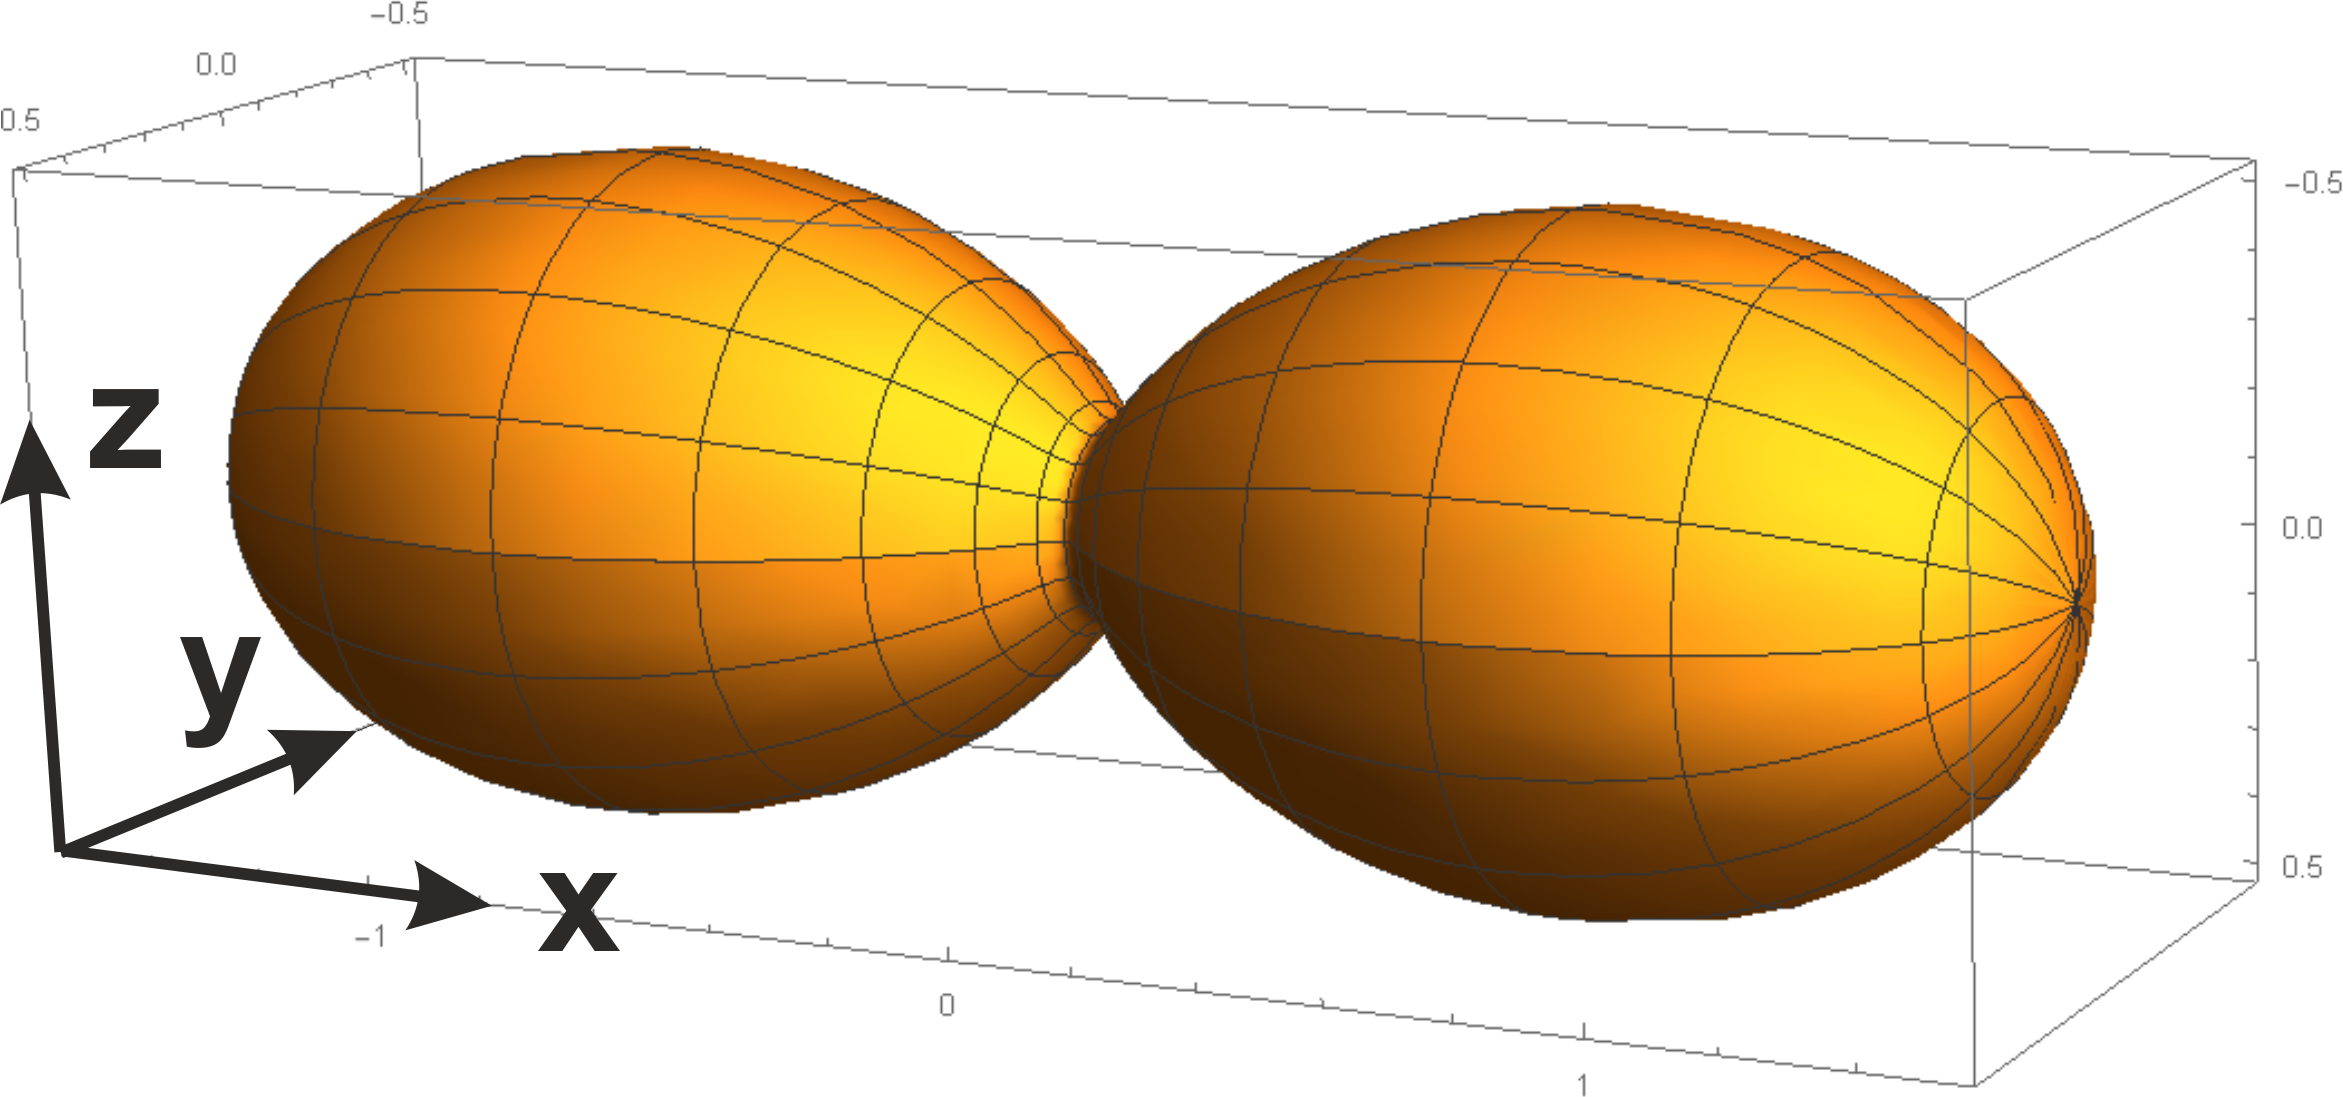
\includegraphics[width=0.55\textwidth]{../images/form_factor/cylindrical_obj/pOnsager(3).png}}
\hfill
\subfigure[Onsager orientation distribution for $\kappa=-3$. ]{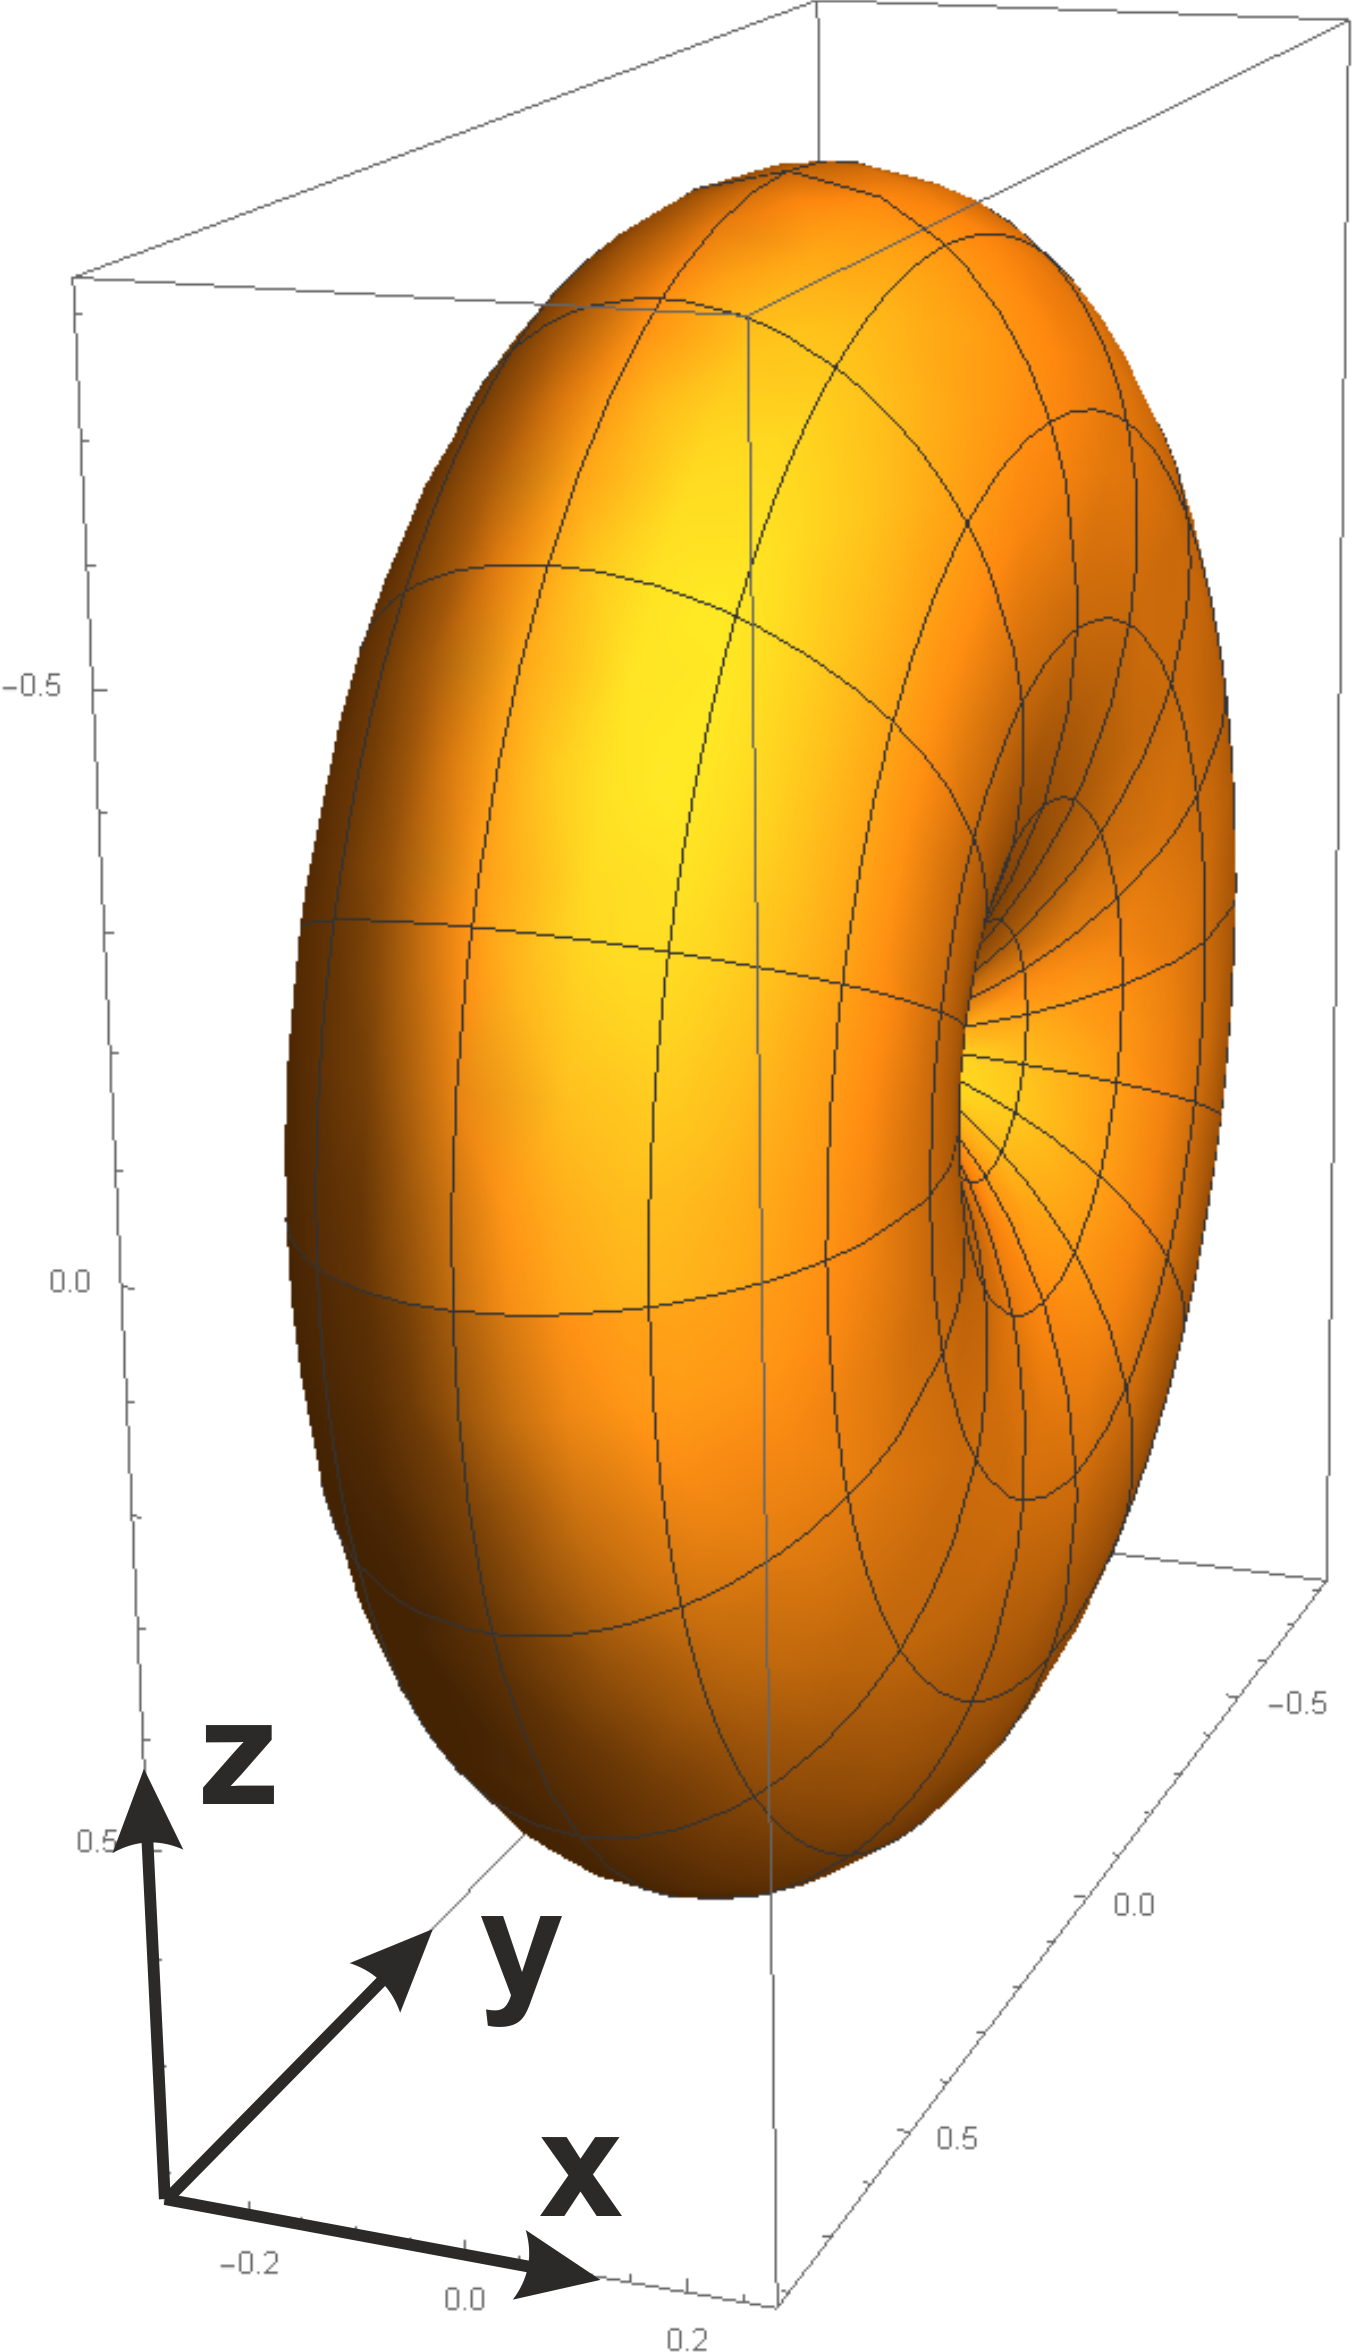
\includegraphics[width=0.4\textwidth]{../images/form_factor/cylindrical_obj/pOnsager(-3).png}}
\caption{Orientation distributions are are all independent on $\phi$ and have for $\kappa>0$ a positive order parameter, i.e. the most probable orientation is in the $\mathbf{x}$-direction and for $\kappa<0$ a negative order parameter, i.e. the most probable orientation lies in the $\mathbf{zy}$-plane}
\label{fig:pOnsager3D}
\end{figure}

\begin{figure}[htb]
\begin{center}
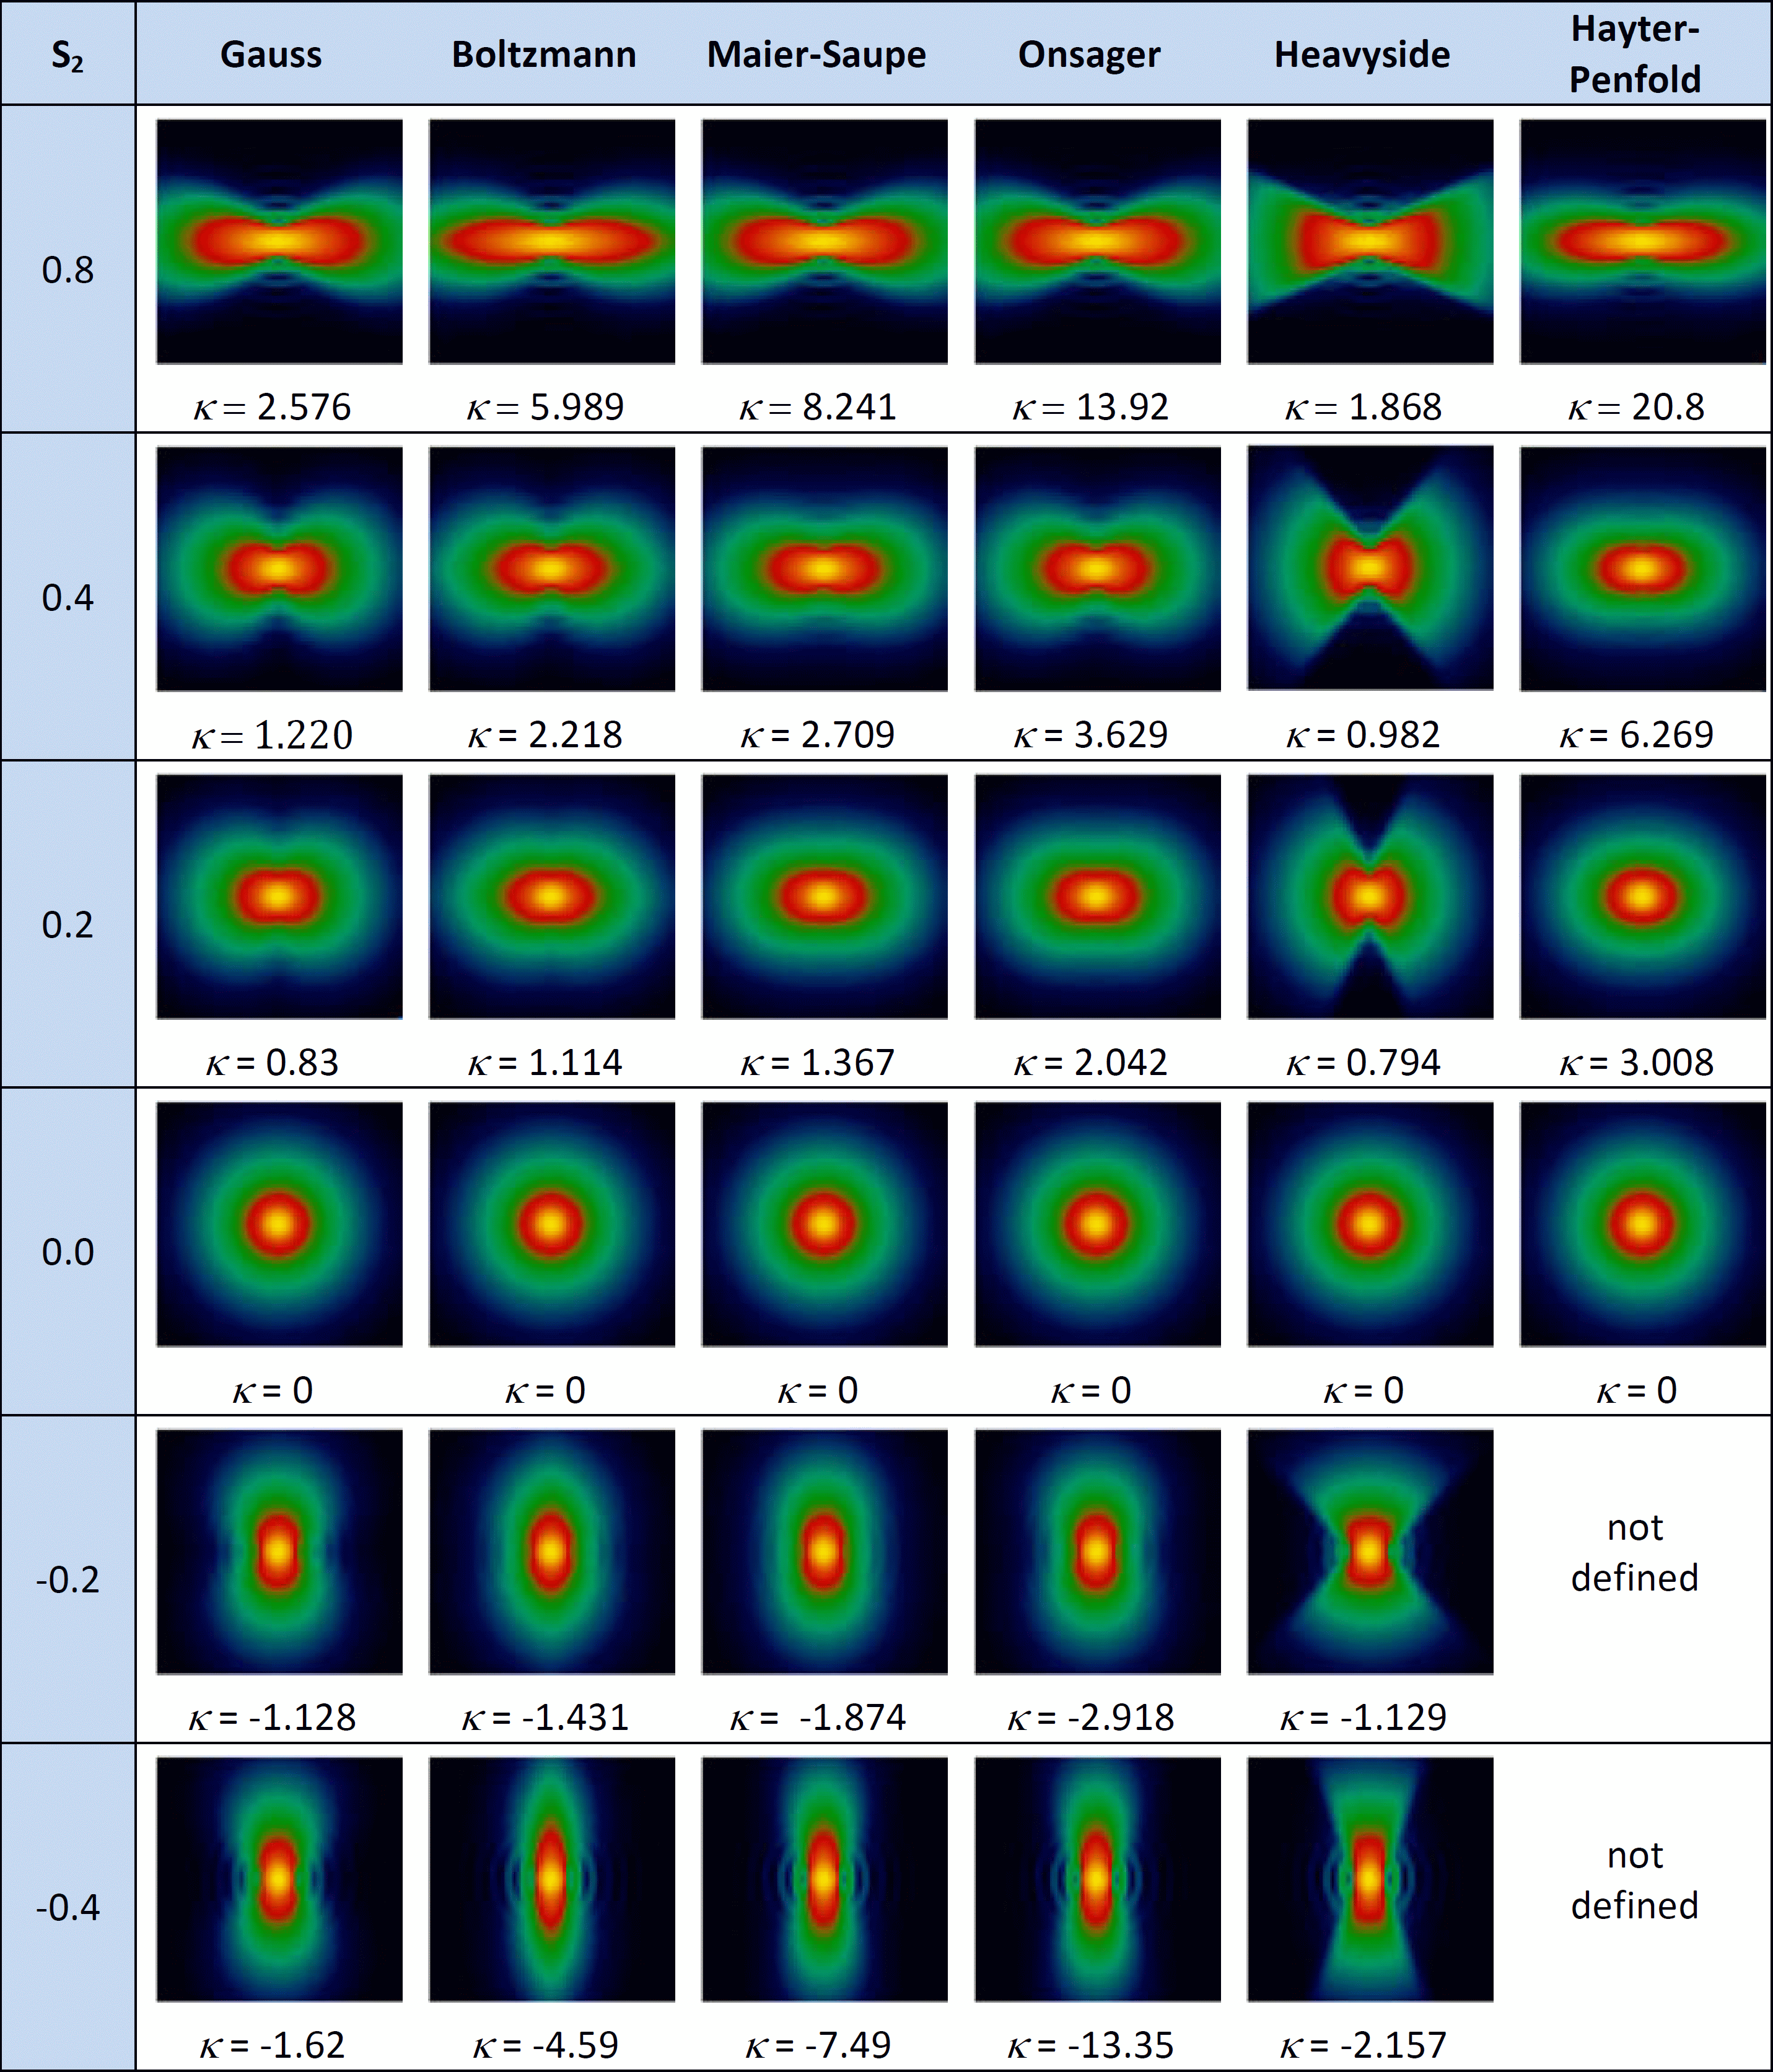
\includegraphics[width=0.95\textwidth]{../images/form_factor/cylindrical_obj/pXXXcomparison.png}
\end{center}
\caption{comparison of different orientation distributions with the same order parameter.}
\label{fig:S2_comparision}
\end{figure}

The order parameter for the Hayter-Penfold orientation distribution has been calculated by performing first a coordination transformation of the polar coordinates with $\mathbf{z}$ being the polar axis to coordination system with a polar axis pointing into the direction of the most probable orientation. The order parameter $S_2(\kappa)$ in eq.\ \ref{eq:S2kappa} is then calculated in this new polar coordinate system.

The form factors additional contain already a size distribution to profit from the speed enhancement by using a specialized multidimensional integration routine. The size distribution is included as
\begin{align} 
I(Q) &= \int_0^\infty \mathrm{LogNorm}(\nu,\sigma,1) I_\mathrm{p.a.CylShell}(Q,R\nu,\Delta R\nu,L\nu) \, \mathrm{d}\nu \\
\end{align}
and
\begin{align}
I(Q) &= \int_0^\infty \mathrm{LogNorm}(\nu,\sigma,1) I_\mathrm{p.a.EllShell}(Q,R_\mathrm{p}\nu,\Delta R\nu,R_\mathrm{e}\nu) \, \mathrm{d}\nu
\end{align}
 with 
\begin{align}
\mathrm{LogNorm}(\nu,\sigma,\mu) &= \frac{1}{\sqrt{2\pi}\sigma}\frac{1}{\nu} \exp\left(-\frac{(\ln(\nu/\mu))^2}{2\sigma^2}\right)
\end{align}

%%%%%%%%%%%%%%%%%%%%%%%%%%%%%%%%%%%%%%%%%%%%%%%%%%%%%%%%%%%%%%%%%%%%%%%%%%%%%%%%%%%%%%%%%%%%%%%%%%%%%%%%%
\clearpage
\subsubsection{Maier-Saupe orientation distribution} ~\\

\begin{figure}[htb]
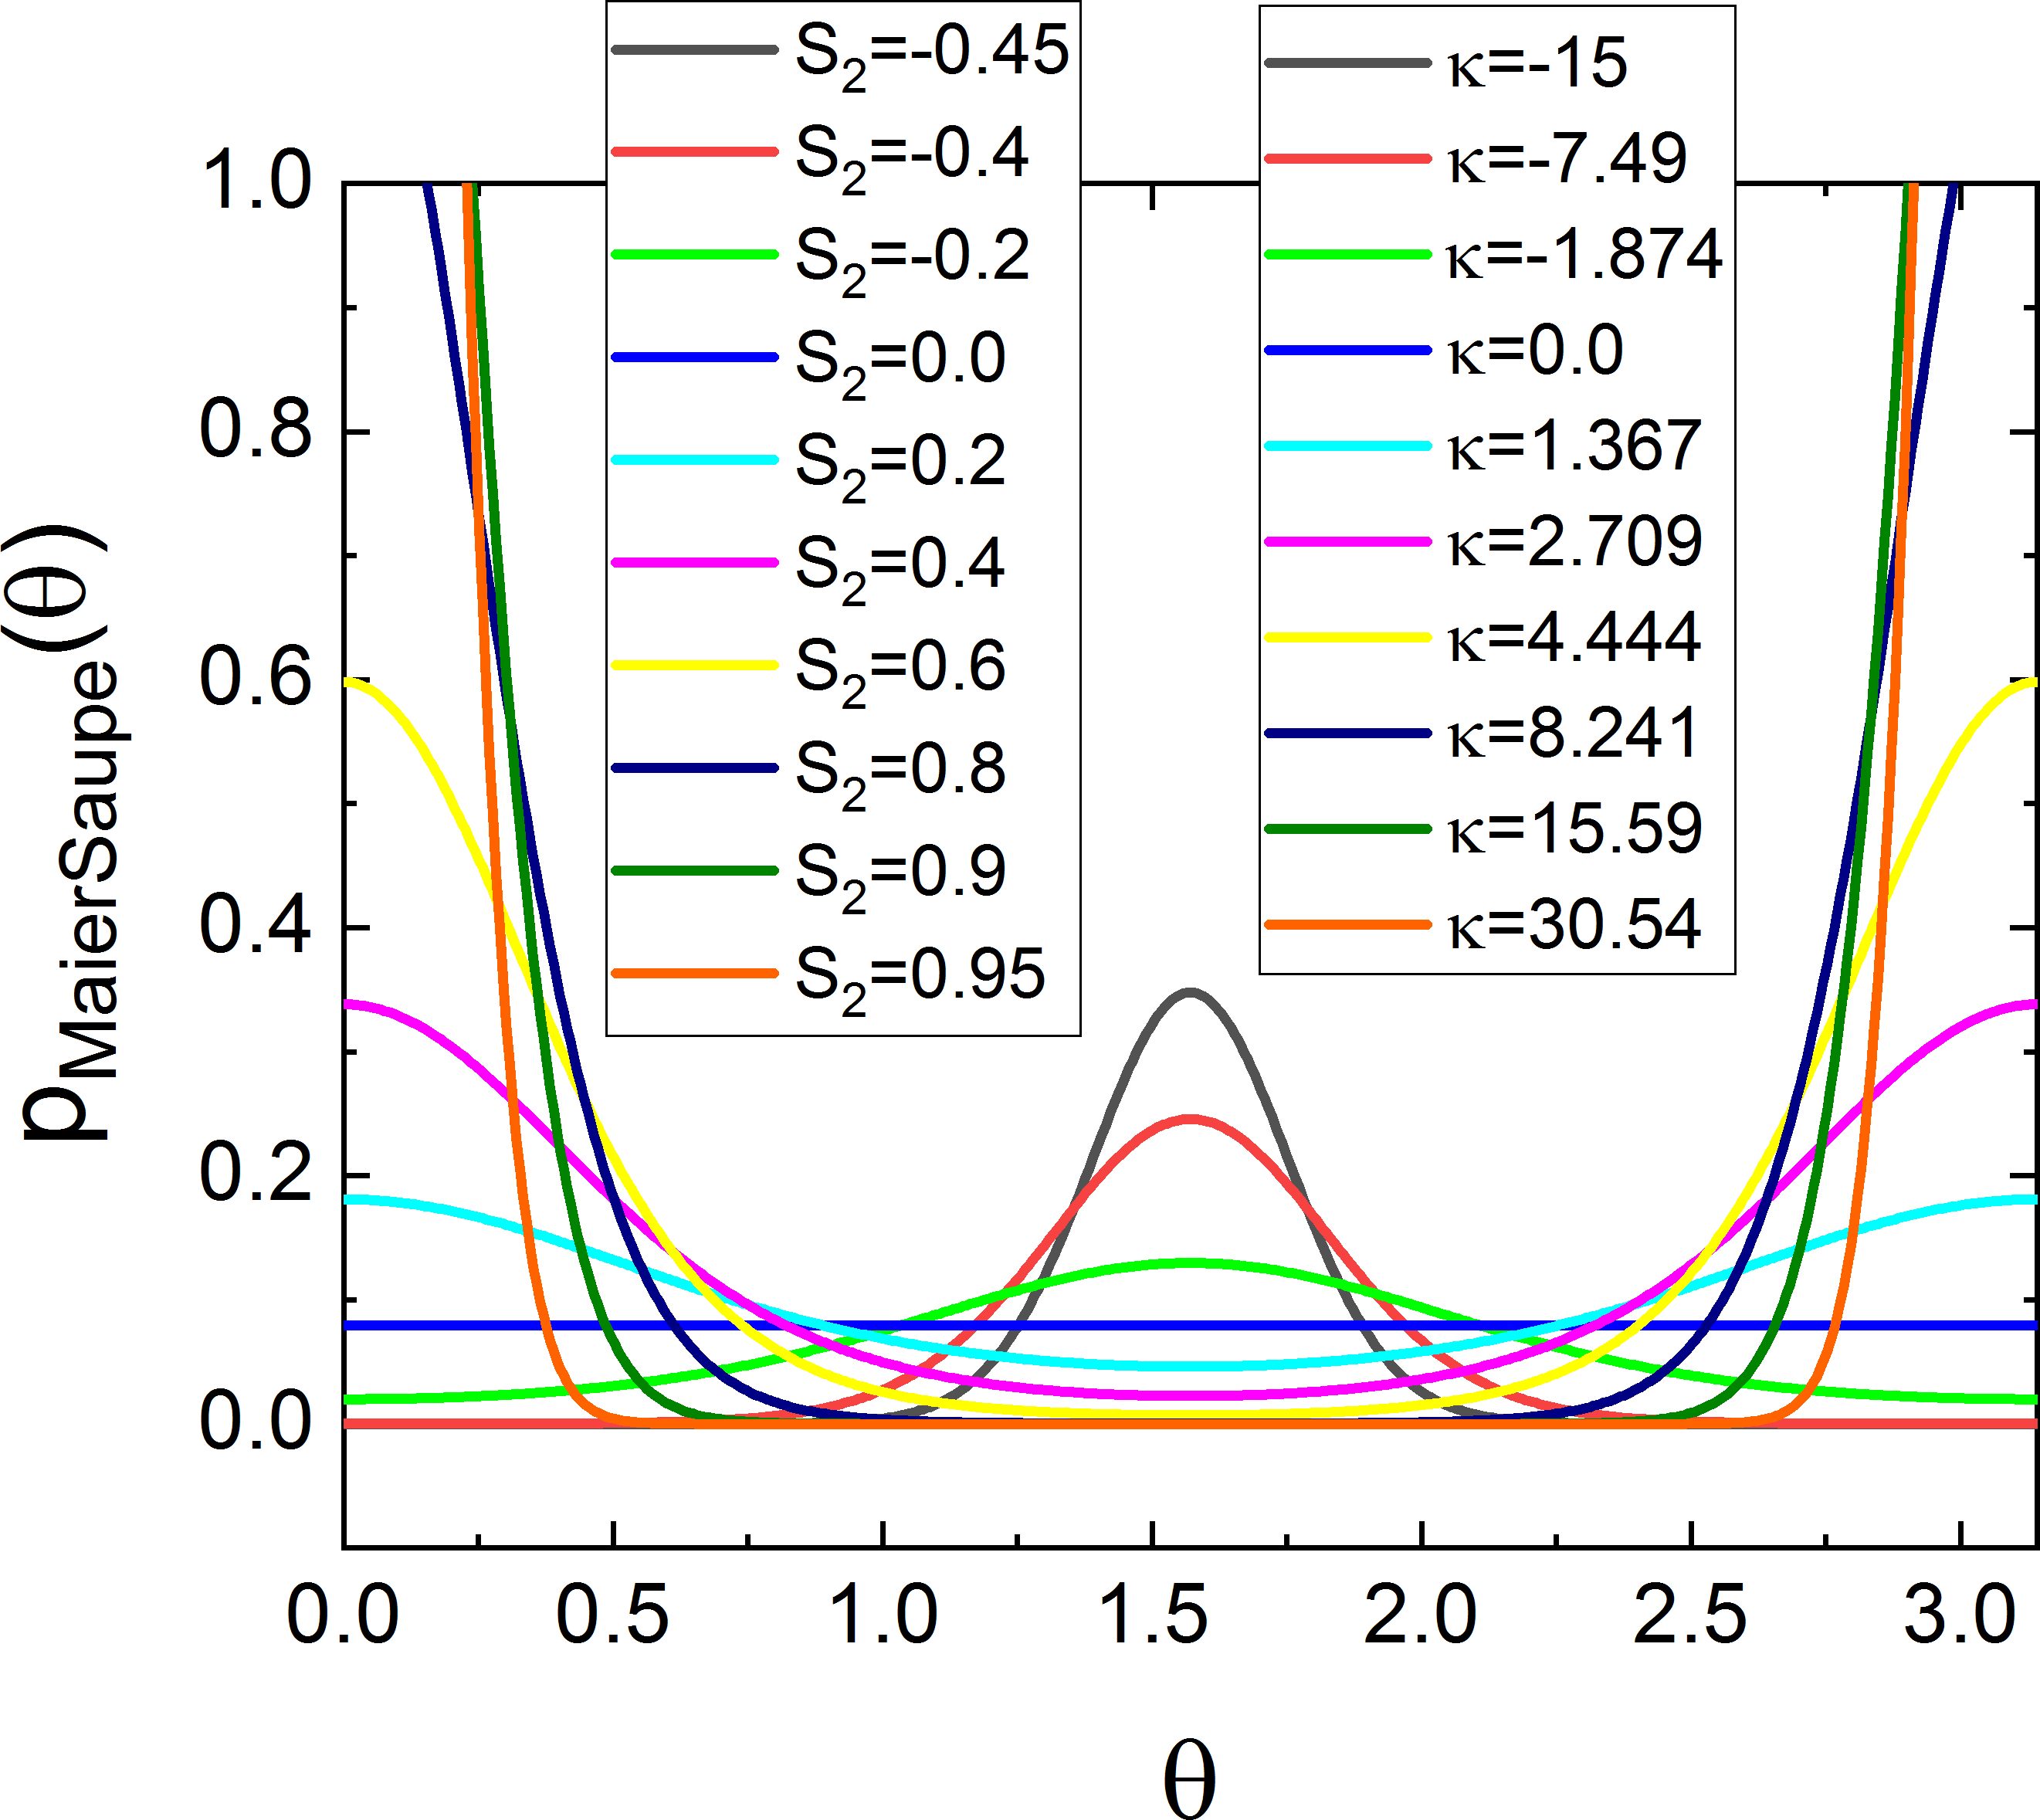
\includegraphics[width=0.75\textwidth]{../images/form_factor/cylindrical_obj/pMaierSaupeGr.png}
\caption{Maier-Saupe orientation distribution $p_\mathrm{MS}(\theta,\kappa)$ for different values of $\kappa$, resulting in an order parameter as listed in table \ref{tab:kappas}.}
\label{fig:pMaierSaupeGr}
\end{figure}

\begin{align}
p(\theta,\phi;\kappa) & = \frac{1}{c_\mathrm{MS}}\exp\left(\kappa \cos^2\theta\right)
\end{align}
with
\begin{align}
c_\mathrm{MS} &=
\begin{cases}
\displaystyle
4\pi\exp(\kappa) \frac{\mathrm{D}\left(\sqrt{\kappa}\right)}{\sqrt{\kappa}}   &\mathrm{for~} \kappa > 0 \\[5mm]
\displaystyle
2\pi \sqrt{\pi} \frac{\mathrm{erf}\left(\sqrt{\abs{\kappa}}\right)}{\sqrt{\abs{\kappa}}}  &\mathrm{for~} \kappa < 0 \\[2mm]
\displaystyle
4\pi                                                                                      &\mathrm{for~} \kappa = 0
\end{cases}
\end{align}
with $D(x)$ being Dawson's integral $D(x)=e^{-x^2}\int_0^x e^{y^2} \mathrm{d}y = \frac12\sqrt{\pi}e^{-x^2}\mathrm{erfi}(x)$

\vspace{5mm}

\underline{Input Parameters for model \texttt{Sheared Cylinders (Maier-Saupe)}:}\\
\begin{description}
\item[\texttt{R}] radius of cylinders $R$
\item[\texttt{t}] shell thickness $t$
\item[\texttt{L}] cylinder length $L$
\item[\texttt{eta\_core}] scattering length density of cylinder core $\eta_\mathrm{core}$
\item[\texttt{eta\_shell}] scattering length density of cylinder shell $\eta_\mathrm{shell}$
\item[\texttt{eta\_solv}] scattering length density of solvent $\eta_\mathrm{solv}$
\item[\texttt{psi}] direction of scattering vector on the detector $\psi$
\item[{\texttt{sigma}}] width parameter of lognormal size distribution $\sigma$
\item[{\texttt{kappa}}] orientation distribution parameter $\kappa$
\end{description}

\vspace{5mm}

\underline{Input Parameters for model \texttt{Sheared Spheroids (Maier-Saupe)}:}\\
\begin{description}
\item[\texttt{R\_equatorial}] equatorial semi-axes of spheroids $R_\mathrm{e}$
\item[\texttt{t}] shell thickness $t$
\item[\texttt{R\_polar}] polar semi-axis of spheroids $R_\mathrm{p}$
\item[\texttt{eta\_core}] scattering length density of cylinder core $\eta_\mathrm{core}$
\item[\texttt{eta\_shell}] scattering length density of cylinder shell $\eta_\mathrm{shell}$
\item[\texttt{eta\_solv}] scattering length density of solvent $\eta_\mathrm{solv}$
\item[\texttt{psi}] direction of scattering vector on the detector $\psi$
\item[{\texttt{sigma}}] width parameter of lognormal size distribution $\sigma$
\item[{\texttt{kappa}}] orientation distribution parameter $\kappa$
\end{description}

\vspace{5mm}

\underline{Note:}
\begin{itemize}
\item The size distribution is taken simultaneously over all parameters $R$, $t$, $L$, and $R_\mathrm{e}$, $t$, $R_\mathrm{p}$ respectively, so that their aspect ratios always stay constant.
\end{itemize}
%%%%%%%%%%%%%%%%%%%%%%%%%%%%%%%%%%%%%%%%%%%%%%%%%%%%%%%%%%%%%%%%%%%%%%%%%%%%%%%%%%

\newpage
\subsubsection{Onsager orientation distribution} ~\\

\begin{figure}[htb]
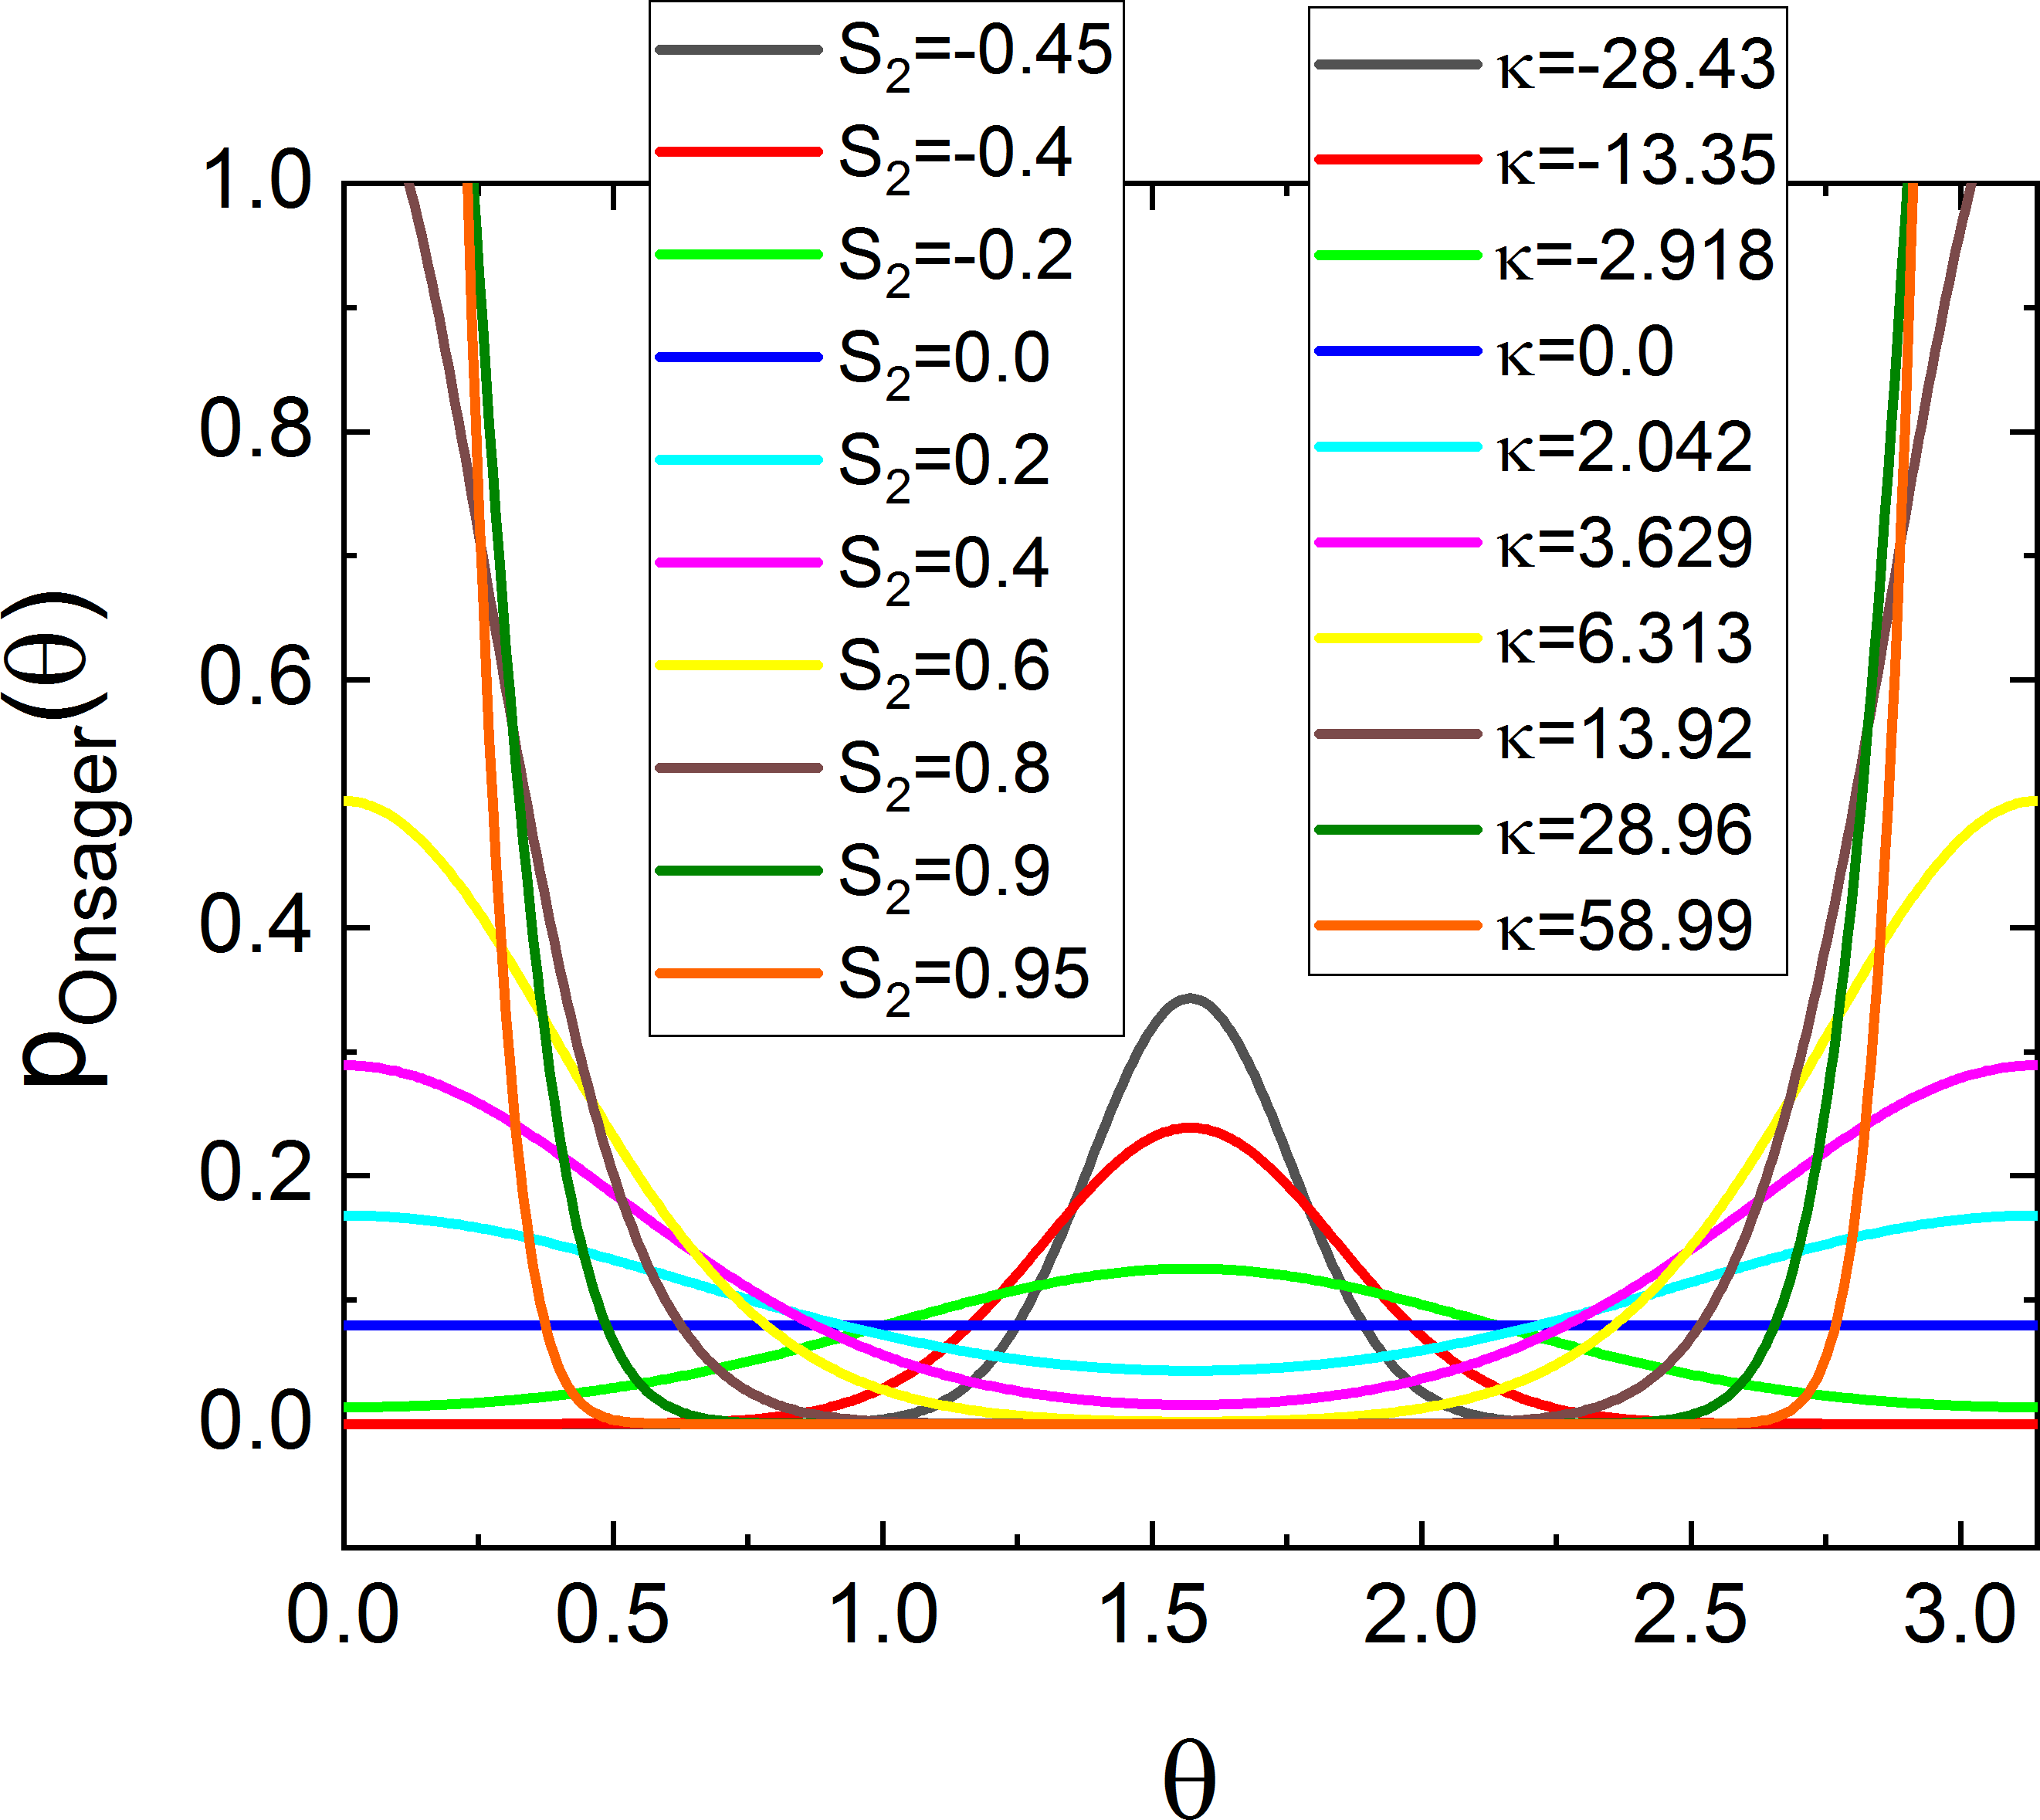
\includegraphics[width=0.75\textwidth]{../images/form_factor/cylindrical_obj/pOnsagerGr.png}
\caption{Onsager orientation distribution $p_\mathrm{O}(\theta,\kappa)$ for different values of $\kappa$, resulting in an order parameter as listed in table \ref{tab:kappas}.}
\label{fig:pOnsagerGr}
\end{figure}

\begin{align}
p_\mathrm{O}(\theta,\phi;\kappa) & =
\begin{cases} \displaystyle
\frac{\kappa \cosh\left(\kappa \cos(\theta)\right)}{4\pi \sinh(\kappa)}      &\mathrm{for~} \kappa \geq 0 \\[5mm]
 \displaystyle
\frac{\cosh\left(\abs{\kappa} \sin(\theta)\right)}{2\pi^2 L_1(\abs{\kappa})}  &\mathrm{for~} \kappa < 0
\end{cases}
\end{align}
where $L_\nu(x)$ is the modified Struve function.

\vspace{5mm}

\underline{Input Parameters for model \texttt{Sheared Cylinders (Onsager)}:}\\
\begin{description}
\item[\texttt{R}] radius of cylinders $R$
\item[\texttt{t}] shell thickness $t$
\item[\texttt{L}] cylinder length $L$
\item[\texttt{eta\_core}] scattering length density of cylinder core $\eta_\mathrm{core}$
\item[\texttt{eta\_shell}] scattering length density of cylinder shell $\eta_\mathrm{shell}$
\item[\texttt{eta\_solv}] scattering length density of solvent $\eta_\mathrm{solv}$
\item[\texttt{psi}] direction of scattering vector on the detector $\psi$
\item[{\texttt{sigma}}] width parameter of lognormal size distribution $\sigma$
\item[{\texttt{kappa}}] orientation distribution parameter $\kappa$
\end{description}

\vspace{5mm}

\underline{Input Parameters for model \texttt{Sheared Spheroids (Onsager}:}\\
\begin{description}
\item[\texttt{R\_equatorial}] equatorial semi-axes of spheroids $R_\mathrm{e}$
\item[\texttt{t}] shell thickness $t$
\item[\texttt{R\_polar}] polar semi-axis of spheroids $R_\mathrm{p}$
\item[\texttt{eta\_core}] scattering length density of cylinder core $\eta_\mathrm{core}$
\item[\texttt{eta\_shell}] scattering length density of cylinder shell $\eta_\mathrm{shell}$
\item[\texttt{eta\_solv}] scattering length density of solvent $\eta_\mathrm{solv}$
\item[\texttt{psi}] direction of scattering vector on the detector $\psi$
\item[{\texttt{sigma}}] width parameter of lognormal size distribution $\sigma$
\item[{\texttt{kappa}}] orientation distribution parameter $\kappa$
\end{description}

\vspace{5mm}

\underline{Note:}
\begin{itemize}
\item The size distribution is taken simultaneously over all parameters $R$, $t$, $L$, and $R_\mathrm{e}$, $t$, $R_\mathrm{p}$ respectively, so that their aspect ratios always stay constant.
\end{itemize}
%%%%%%%%%%%%%%%%%%%%%%%%%%%%%%%%%%%%%%%%%%%%%%%%%%%%%%%%%%%%%%%%%%%%%%%%%%%%%%%%%%

\newpage
\subsubsection{Boltzmann orientation distribution} ~\\

\begin{figure}[htb]
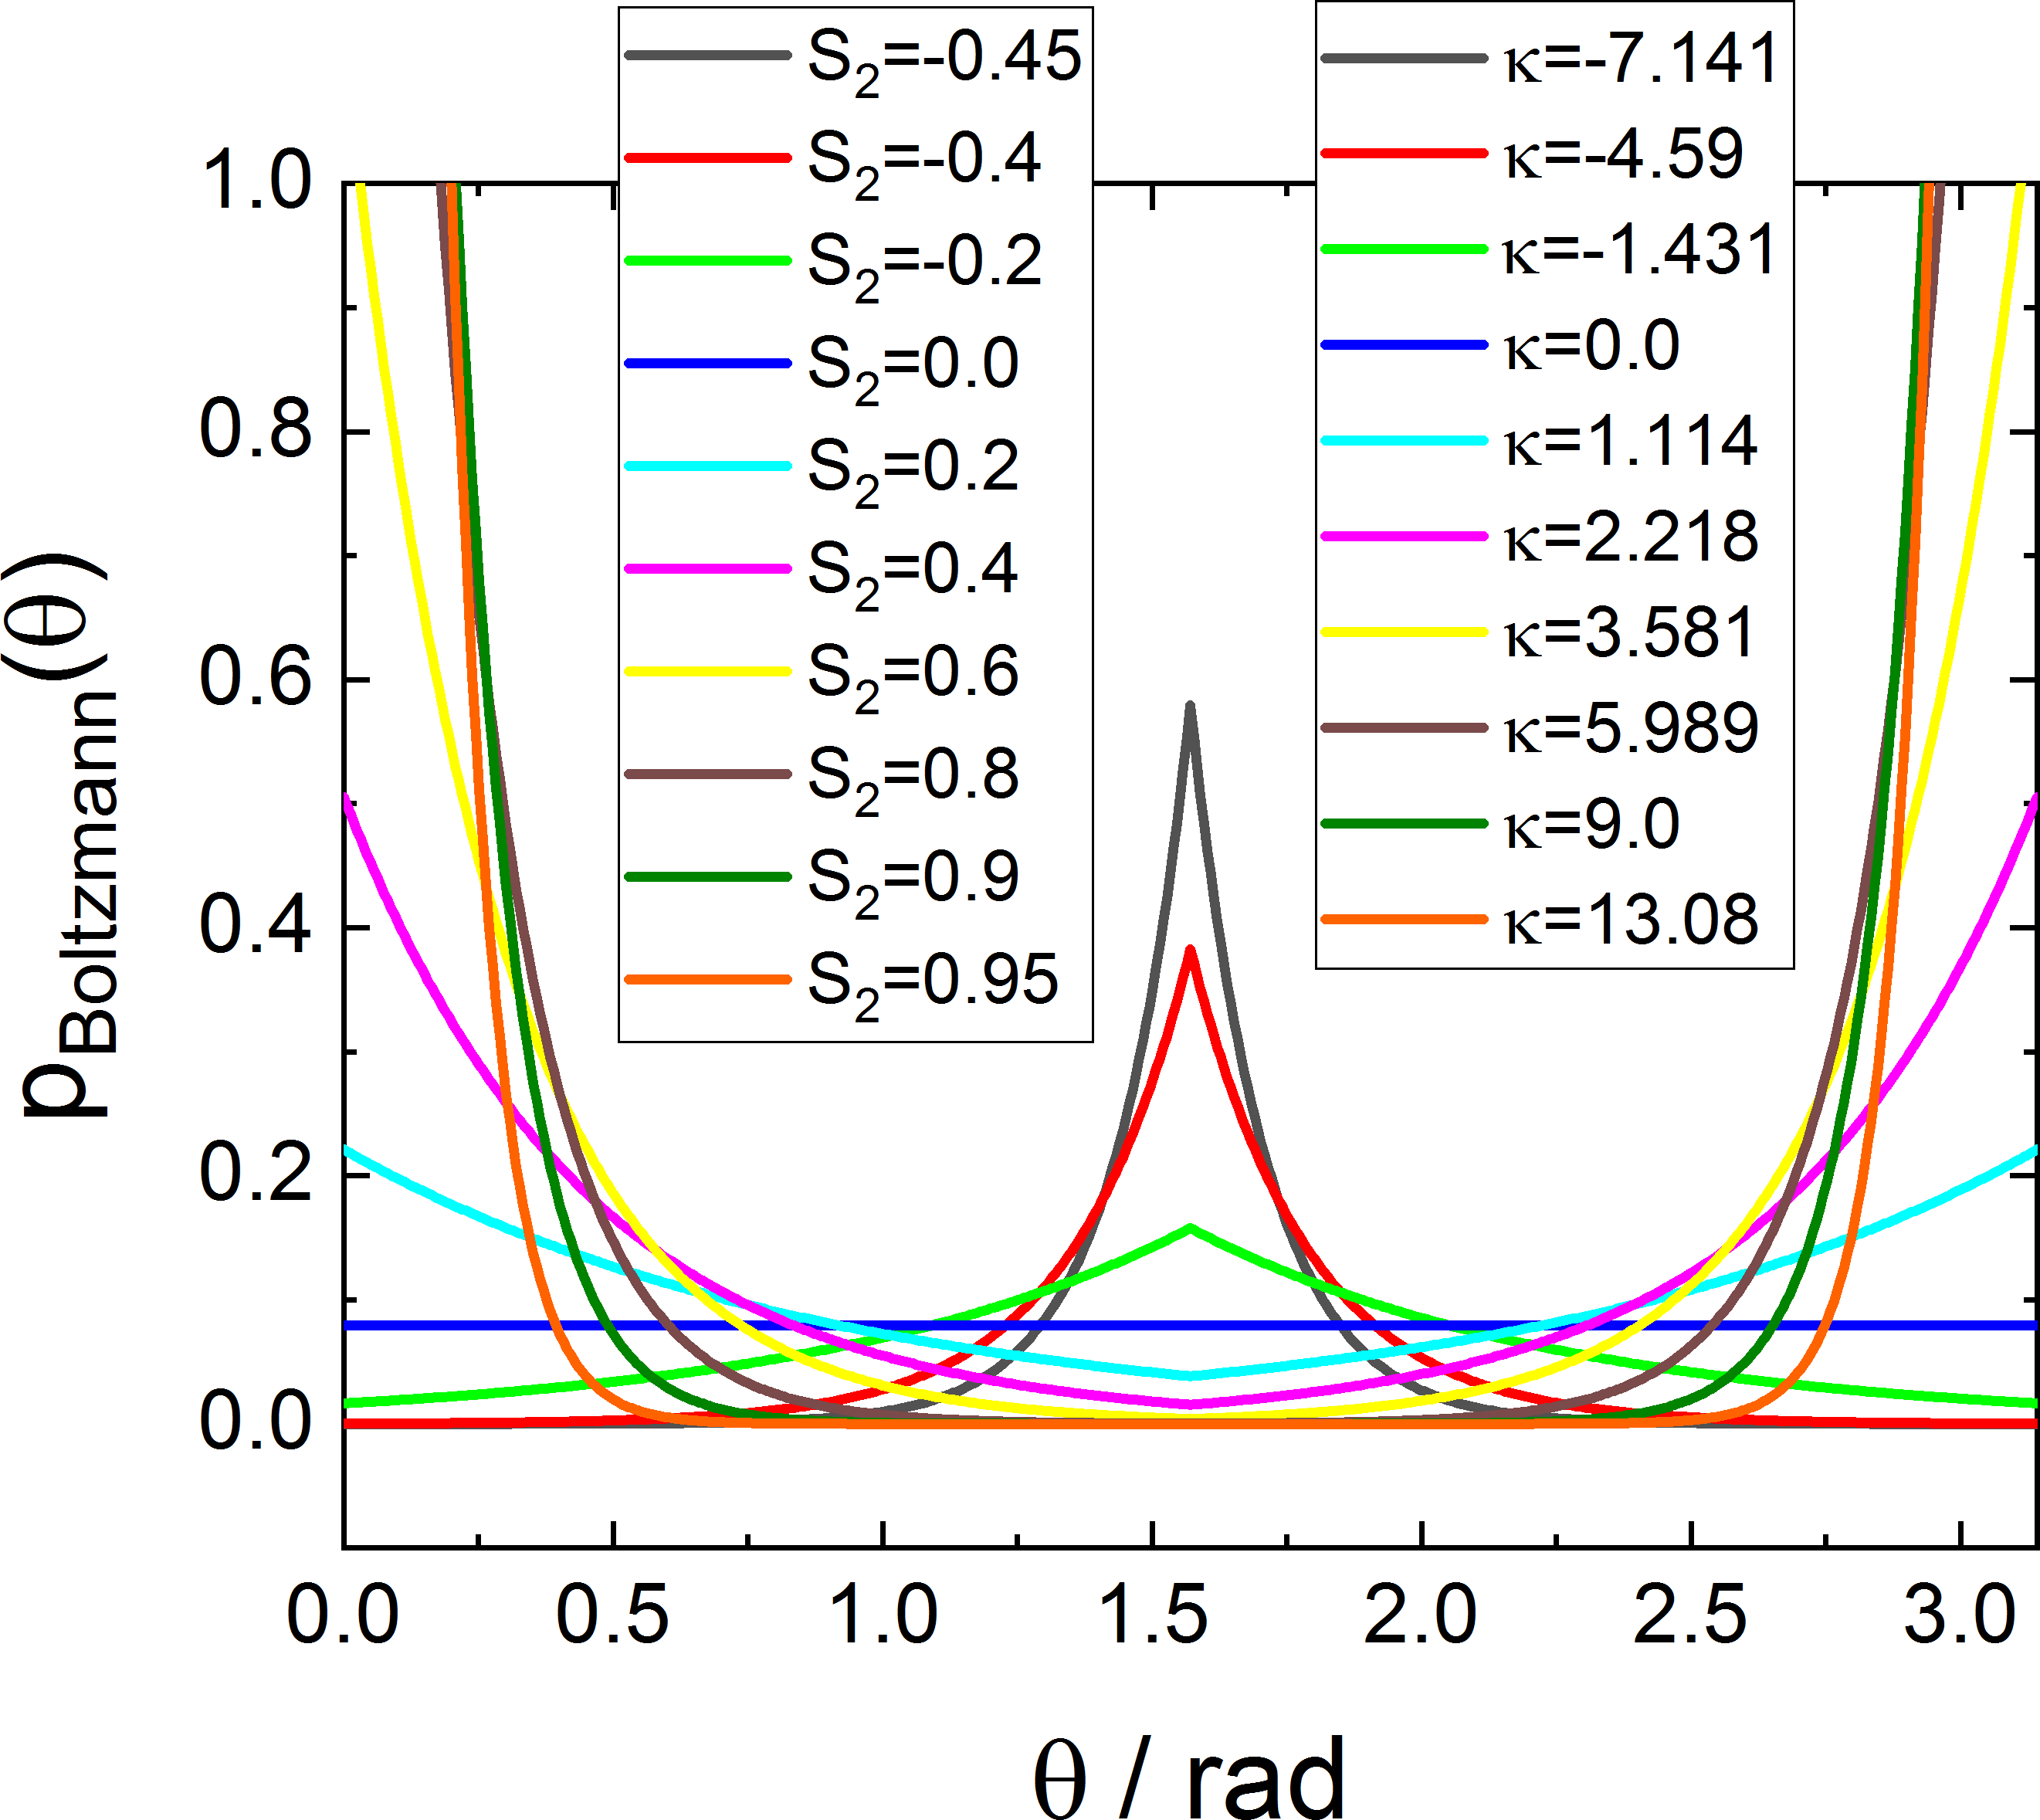
\includegraphics[width=0.75\textwidth]{../images/form_factor/cylindrical_obj/pBoltzmannGr.png}
\caption{Boltzmann orientation distribution $p_\mathrm{B}(\theta,\kappa)$ for different values of $\kappa$, resulting in an order parameter as listed in table \ref{tab:kappas}.}
\label{fig:pBoltzmannGr}
\end{figure}

\begin{align}
p_\mathrm{B}(\theta,\phi;\kappa) & =
\begin{cases}
\displaystyle
\frac{1}{2\pi c_\mathrm{B}}\exp\left(-\theta\kappa\right) & \mathrm{for~}  \theta \leq \frac{\pi}{2}\\[5mm]
\displaystyle
\frac{1}{2\pi c_\mathrm{B}}\exp\left(-(\pi-\theta)\kappa\right) & \mathrm{for~}  \theta > \frac{\pi}{2}
\end{cases}
\end{align}
with
\begin{align}
c_\mathrm{B} &= \frac{2\left(1-\kappa \exp\left(-\frac{\pi}{2}\kappa\right)\right)}{\kappa^2+1}
\end{align}

\vspace{5mm}

\underline{Input Parameters for model \texttt{Sheared Cylinders (Boltzmann)}:}\\
\begin{description}
\item[\texttt{R}] radius of cylinders $R$
\item[\texttt{t}] shell thickness $t$
\item[\texttt{L}] cylinder length $L$
\item[\texttt{eta\_core}] scattering length density of cylinder core $\eta_\mathrm{core}$
\item[\texttt{eta\_shell}] scattering length density of cylinder shell $\eta_\mathrm{shell}$
\item[\texttt{eta\_solv}] scattering length density of solvent $\eta_\mathrm{solv}$
\item[\texttt{psi}] direction of scattering vector on the detector $\psi$
\item[{\texttt{sigma}}] width parameter of lognormal size distribution $\sigma$
\item[{\texttt{kappa}}] orientation distribution parameter $\kappa$
\end{description}

\vspace{5mm}

\underline{Input Parameters for model \texttt{Sheared Spheroids (Boltzmann)}:}\\
\begin{description}
\item[\texttt{R\_equatorial}] equatorial semi-axes of spheroids $R_\mathrm{e}$
\item[\texttt{t}] shell thickness $t$
\item[\texttt{R\_polar}] polar semi-axis of spheroids $R_\mathrm{p}$
\item[\texttt{eta\_core}] scattering length density of cylinder core $\eta_\mathrm{core}$
\item[\texttt{eta\_shell}] scattering length density of cylinder shell $\eta_\mathrm{shell}$
\item[\texttt{eta\_solv}] scattering length density of solvent $\eta_\mathrm{solv}$
\item[\texttt{psi}] direction of scattering vector on the detector $\psi$
\item[{\texttt{sigma}}] width parameter of lognormal size distribution $\sigma$
\item[{\texttt{kappa}}] orientation distribution parameter $\kappa$
\end{description}

\vspace{5mm}

\underline{Note:}
\begin{itemize}
\item The size distribution is taken simultaneously over all parameters $R$, $t$, $L$, and $R_\mathrm{e}$, $t$, $R_\mathrm{p}$ respectively, so that their aspect ratios always stay constant.
\end{itemize}
%%%%%%%%%%%%%%%%%%%%%%%%%%%%%%%%%%%%%%%%%%%%%%%%%%%%%%%%%%%%%%%%%%%%%%%%%%%%%%%%%%

\newpage
\subsubsection{Gaussian orientation distribution}
\label{sect:ShearedCylinderGaussian}
~\\

\begin{figure}[htb]
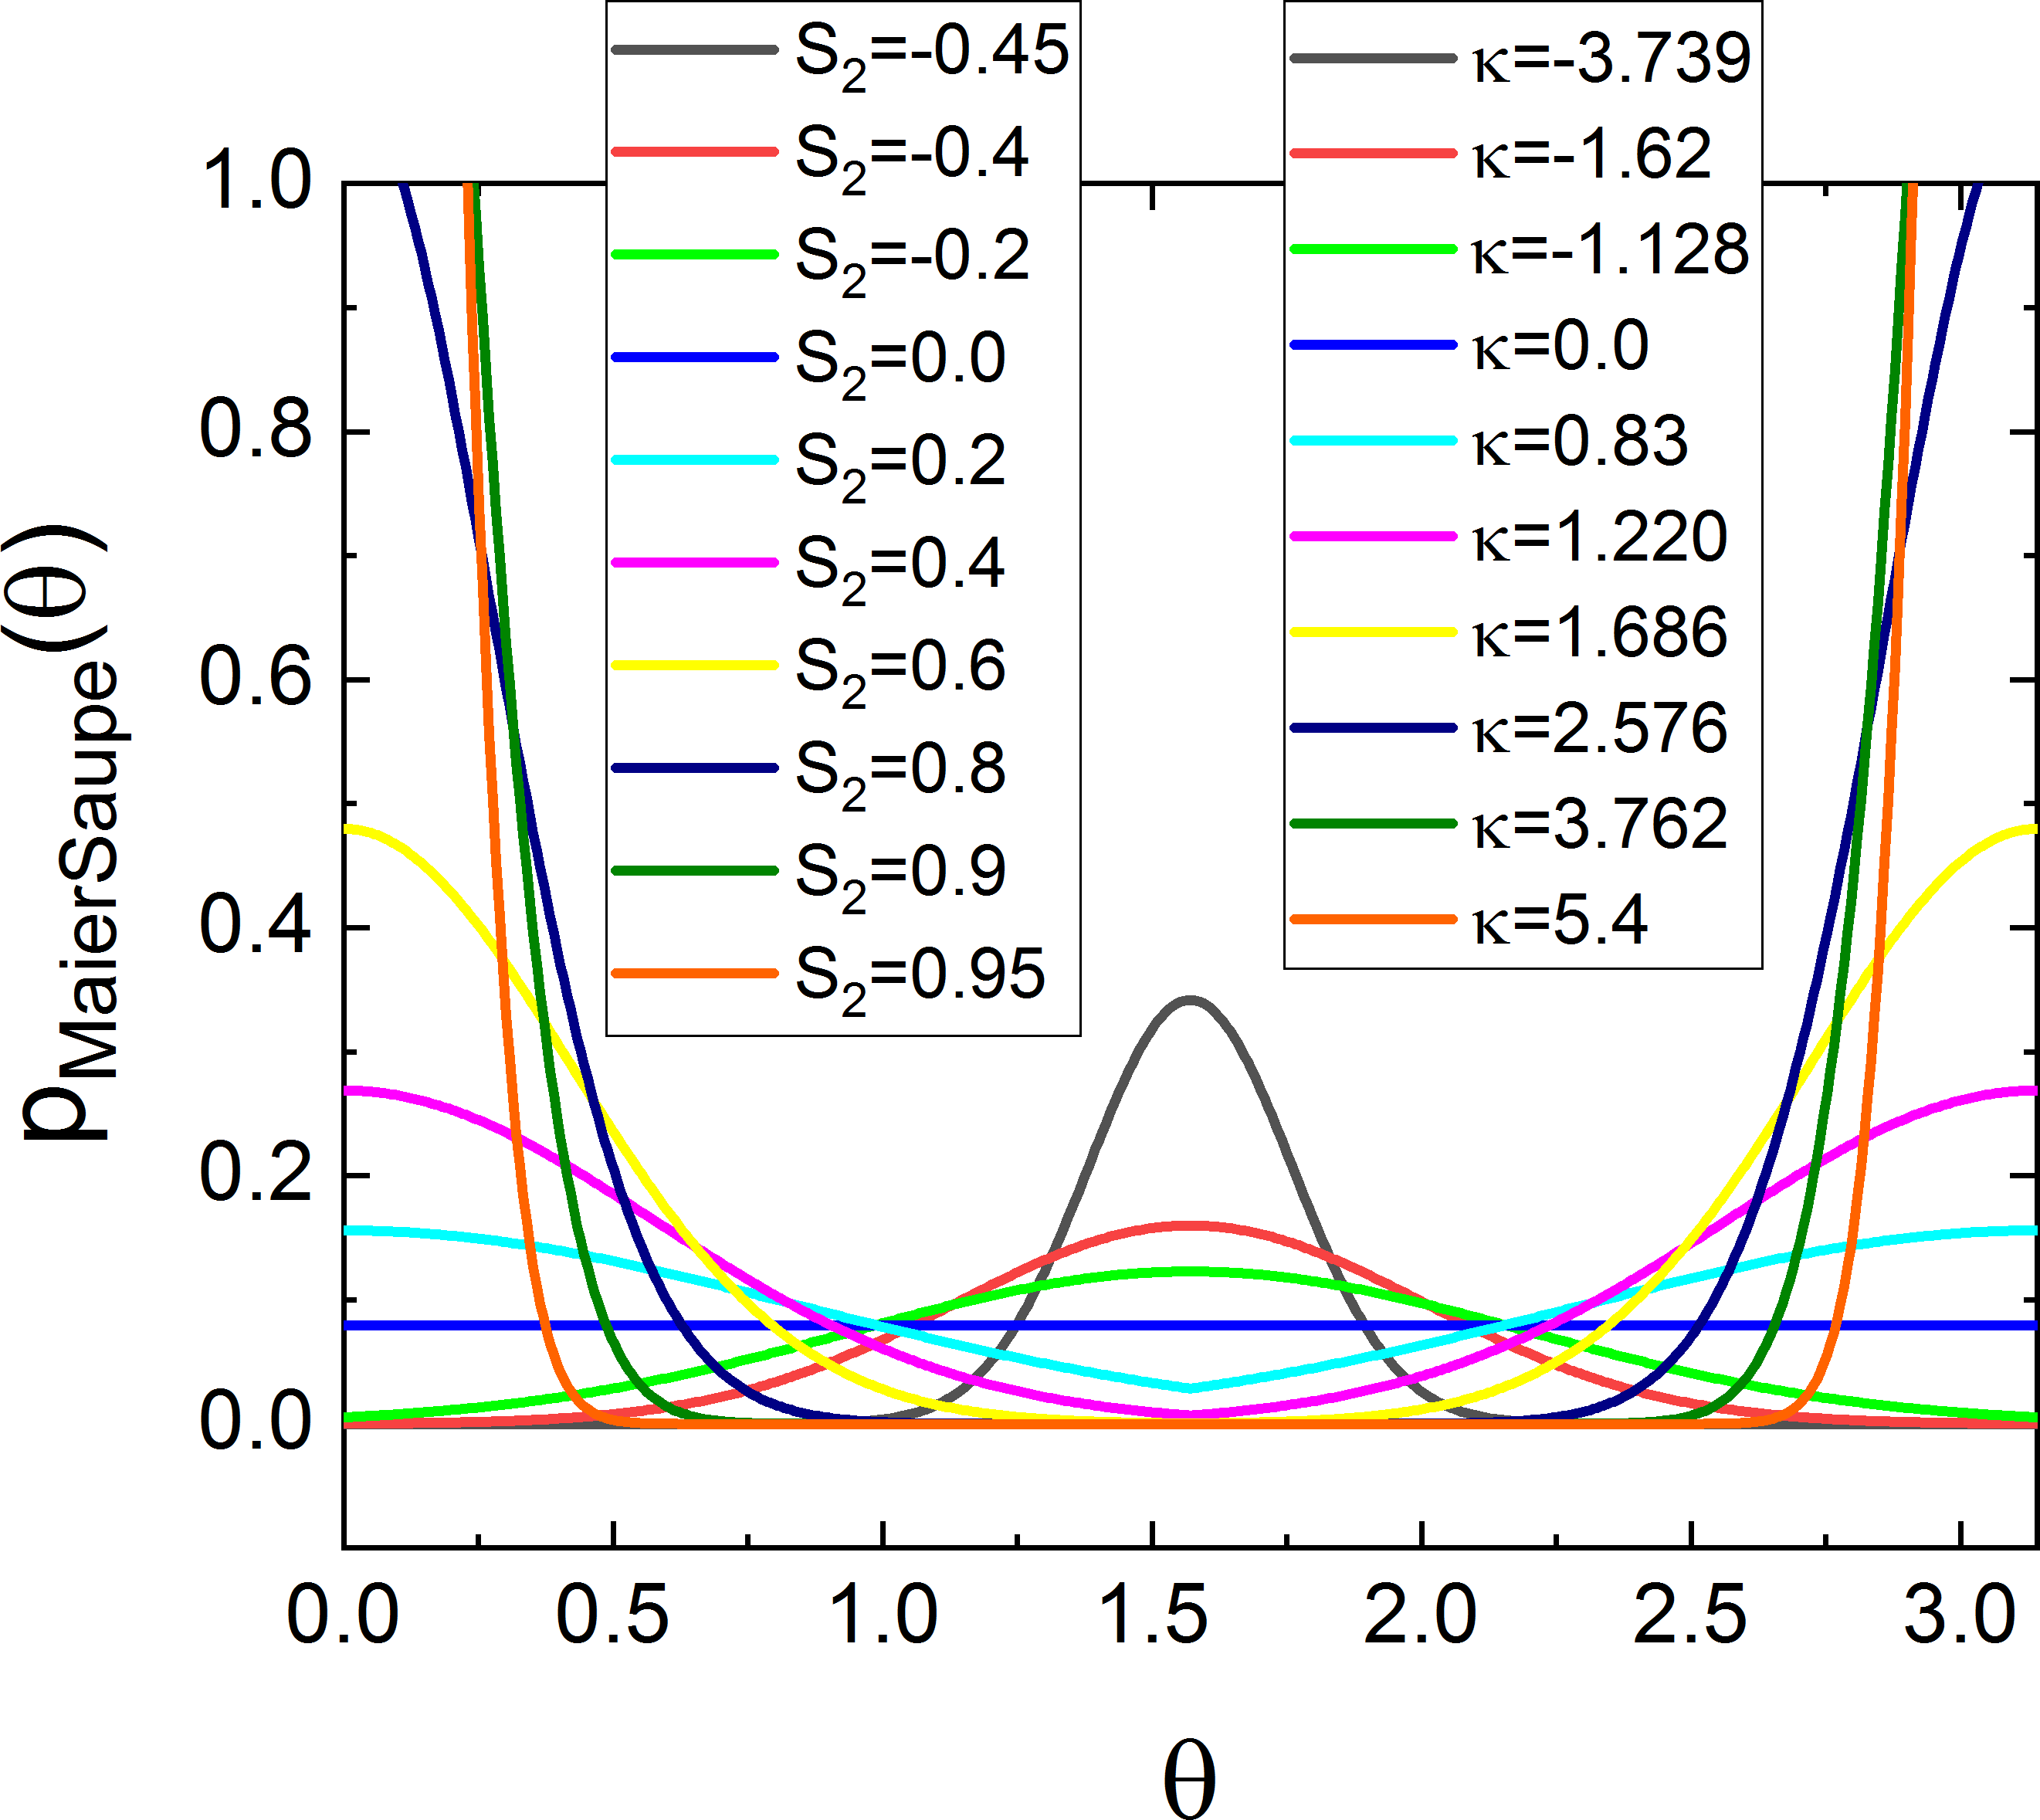
\includegraphics[width=0.75\textwidth]{../images/form_factor/cylindrical_obj/pGaussGr.png}
\caption{Gaussian orientation distribution $p_\mathrm{G}(\theta,\kappa)$ for different values of $\kappa$, resulting in an order parameter as listed in table \ref{tab:kappas}.}
\label{fig:pGaussGr}
\end{figure}

\begin{align}
p_\mathrm{G}(\theta,\phi;\kappa) & =
\begin{cases}
\displaystyle
\frac{1}{2\pi c_\mathrm{G}}\exp\left(-\theta^2\kappa^2\right) & \mathrm{for~} \kappa \geq 0 \mathrm{~and~} \theta \leq \frac{\pi}{2}\\[5mm]
\displaystyle
\frac{1}{2\pi c_\mathrm{G}}\exp\left(-\left(\pi-\theta\right)^2\kappa^2\right) & \mathrm{for~} \kappa \geq 0 \mathrm{~and~} \theta > \frac{\pi}{2}\\[5mm]
\displaystyle
\frac{1}{2\pi c_\mathrm{G}}\exp\left(-\left(\frac{\pi}{2}-\theta\right)^2\abs{\kappa}^2\right) & \mathrm{for~} \kappa < 0
\end{cases}
\end{align}
with
\begin{align}
c_\mathrm{G} & =
\begin{cases}\displaystyle
\frac{D\left(\kappa/2\right)}{\kappa}
           +\frac{\sqrt{\pi}}{2\kappa} e^{-\frac{1}{4\kappa^2}} \Re\left(\mathrm{cerfi}\left(-\frac{1}{2\kappa}+\imath\frac{\pi}{2}\kappa\right) \right)& \mathrm{for~} \kappa \geq 0 \\[5mm]
\displaystyle
\frac{\sqrt{\pi}}{\abs{\kappa}} e^{-\frac{1}{4\kappa^2}} \Im\left(\mathrm{cerfi}\left(-\frac{1}{2\abs{\kappa}}+\imath\frac{\pi}{2}\abs{\kappa}\right) \right) & \mathrm{for~} \kappa < 0
\end{cases}
\end{align}

\vspace{5mm}

\underline{Input Parameters for model \texttt{Sheared Cylinders (Gauss)}:}\\
\begin{description}
\item[\texttt{R}] radius of cylinders $R$
\item[\texttt{t}] shell thickness $t$
\item[\texttt{L}] cylinder length $L$
\item[\texttt{eta\_core}] scattering length density of cylinder core $\eta_\mathrm{core}$
\item[\texttt{eta\_shell}] scattering length density of cylinder shell $\eta_\mathrm{shell}$
\item[\texttt{eta\_solv}] scattering length density of solvent $\eta_\mathrm{solv}$
\item[\texttt{psi}] direction of scattering vector on the detector $\psi$
\item[{\texttt{sigma}}] width parameter of lognormal size distribution $\sigma$
\item[{\texttt{kappa}}] orientation distribution parameter $\kappa$
\end{description}

\vspace{5mm}

\underline{Input Parameters for model \texttt{Sheared Spheroids (Gauss)}:}\\
\begin{description}
\item[\texttt{R\_equatorial}] equatorial semi-axes of spheroids $R_\mathrm{e}$
\item[\texttt{t}] shell thickness $t$
\item[\texttt{R\_polar}] polar semi-axis of spheroids $R_\mathrm{p}$
\item[\texttt{eta\_core}] scattering length density of cylinder core $\eta_\mathrm{core}$
\item[\texttt{eta\_shell}] scattering length density of cylinder shell $\eta_\mathrm{shell}$
\item[\texttt{eta\_solv}] scattering length density of solvent $\eta_\mathrm{solv}$
\item[\texttt{psi}] direction of scattering vector on the detector $\psi$
\item[{\texttt{sigma}}] width parameter of lognormal size distribution $\sigma$
\item[{\texttt{kappa}}] orientation distribution parameter $\kappa$
\end{description}

\vspace{5mm}

\underline{Note:}
\begin{itemize}
\item The size distribution is taken simultaneously over all parameters $R$, $t$, $L$, and $R_\mathrm{e}$, $t$, $R_\mathrm{p}$ respectively, so that their aspect ratios always stay constant.
\end{itemize}

%%%%%%%%%%%%%%%%%%%%%%%%%%%%%%%%%%%%%%%%%%%%%%%%%%%%%%%%%%%%%%%%%%%%%%%%%%%%%%%%%%

\newpage
\subsubsection{Boxed orientation distribution (HeavisidePi)} ~\\

\begin{figure}[htb]
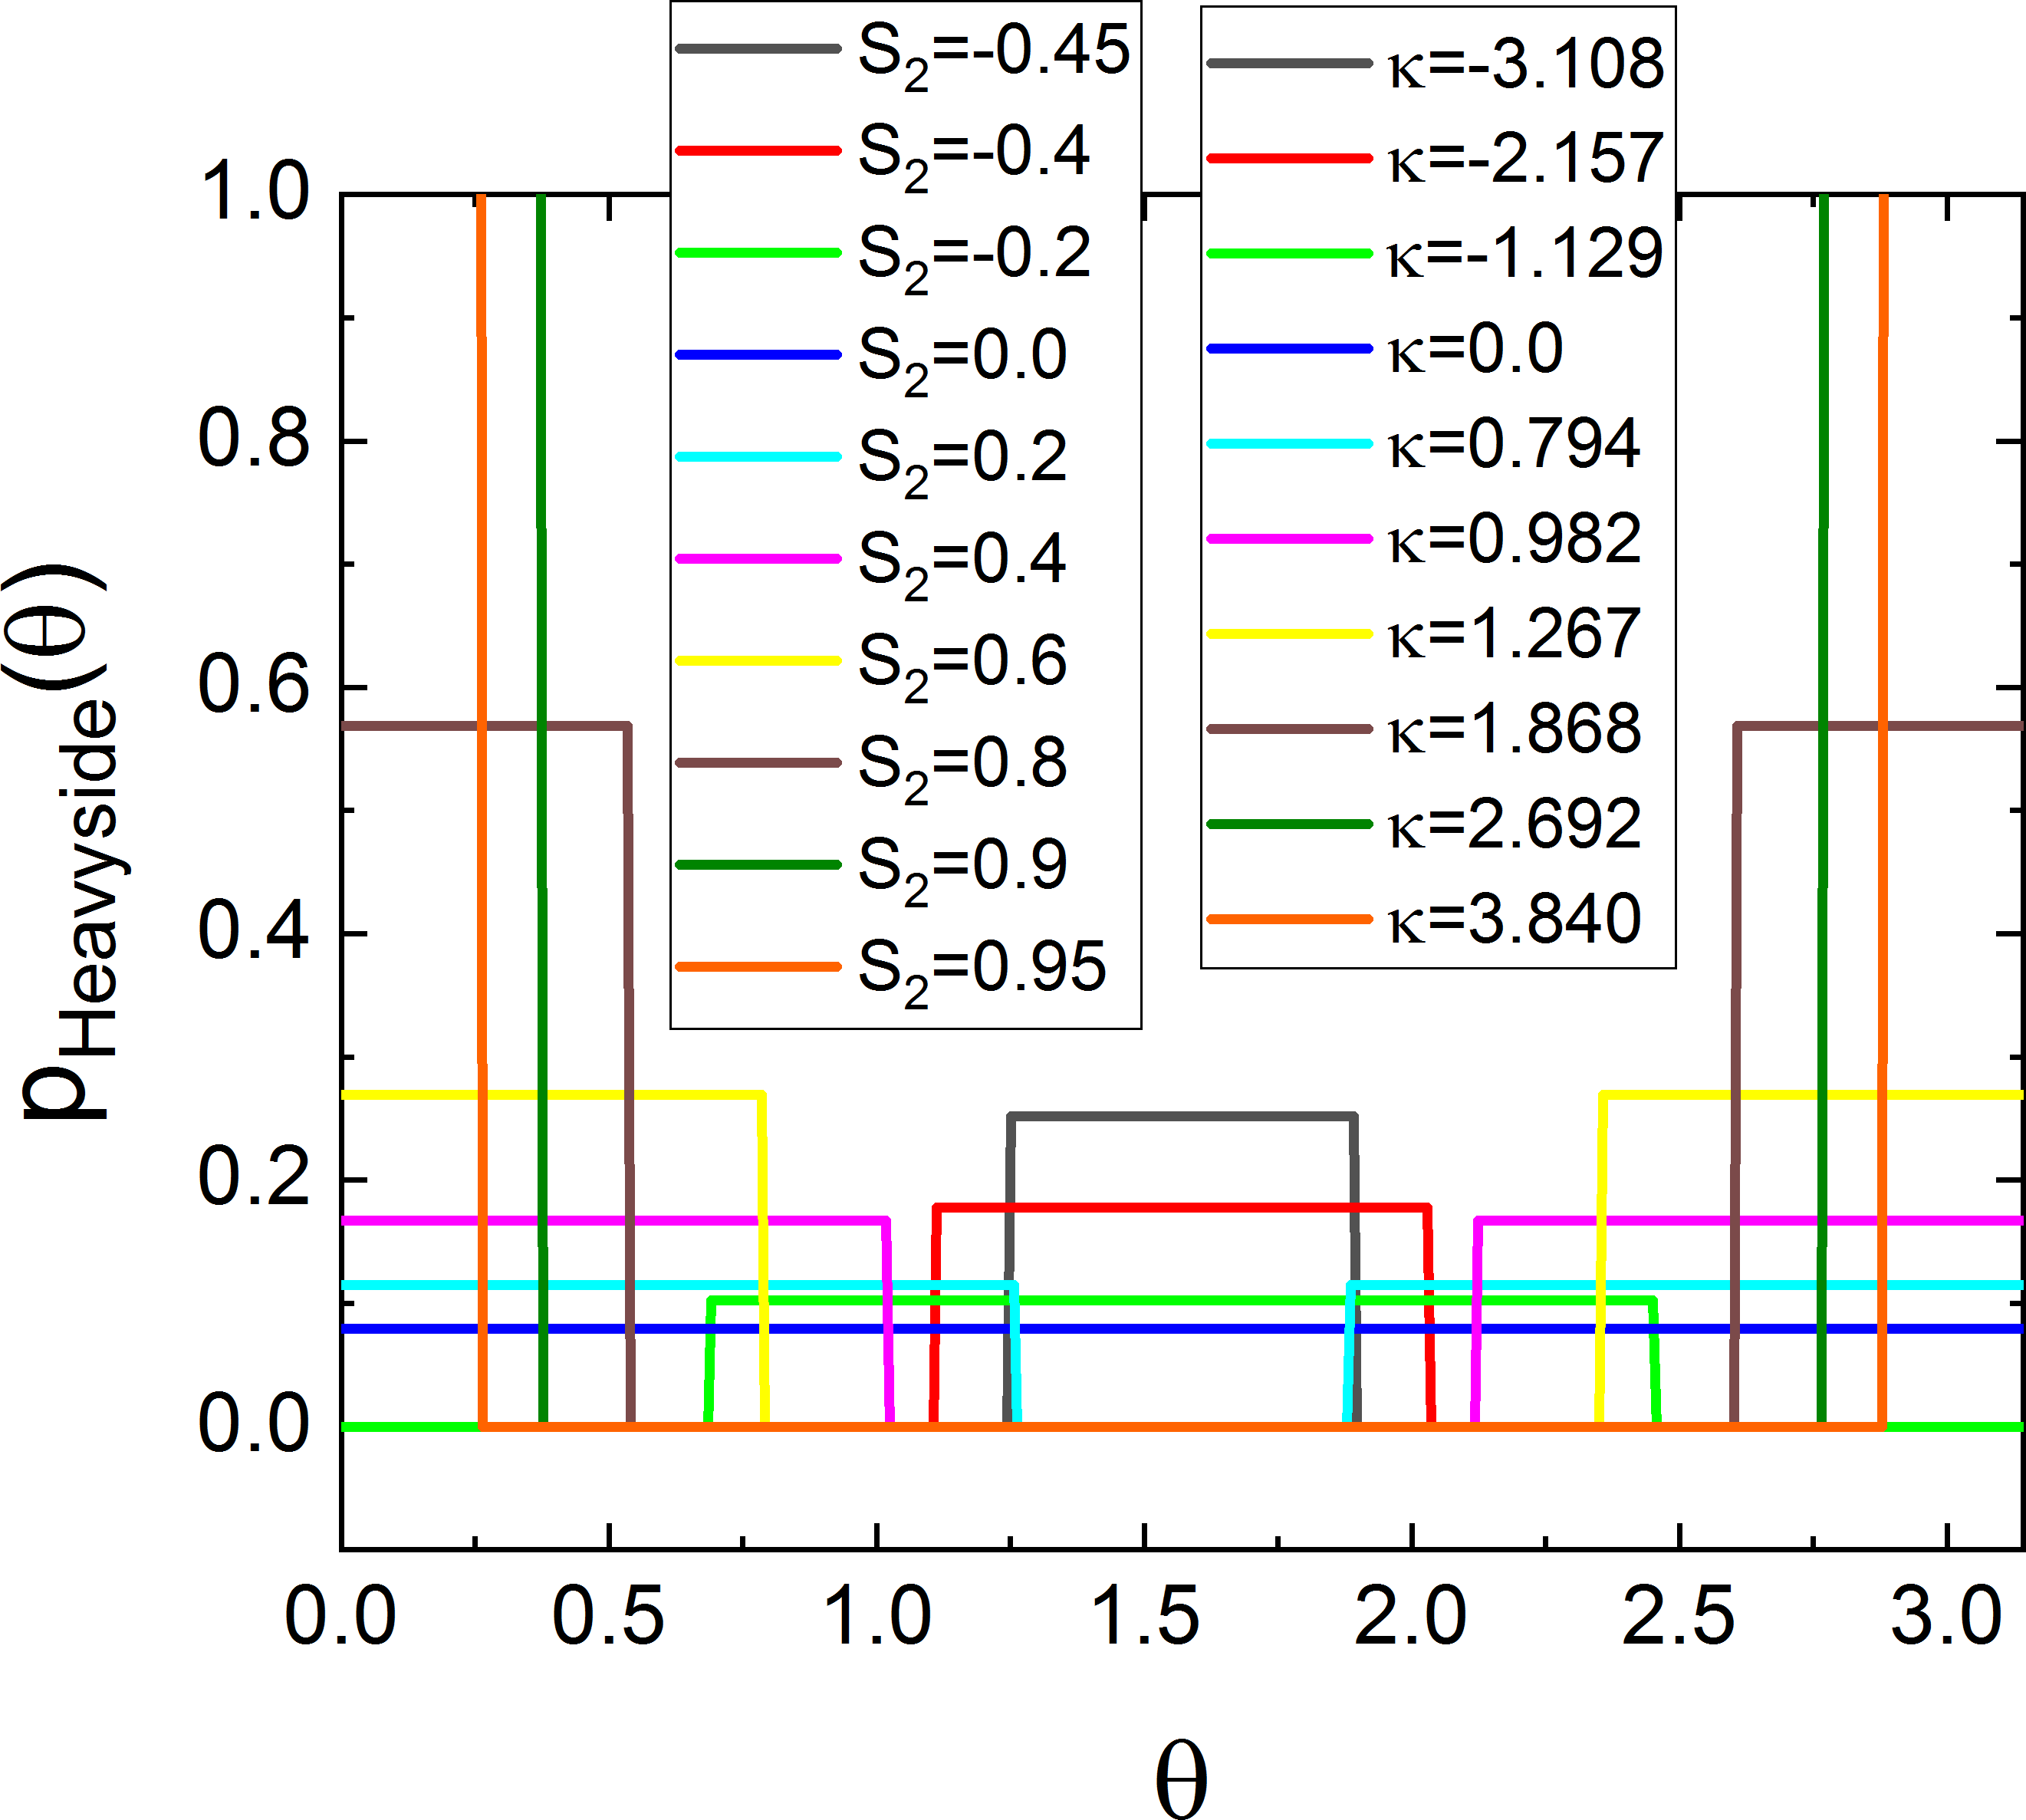
\includegraphics[width=0.75\textwidth]{../images/form_factor/cylindrical_obj/pHeavisideGr.png}
\caption{Heaviside orientation distribution $p_\mathrm{HS}(\theta,\kappa)$ for different values of $\kappa$, resulting in an order parameter as listed in table \ref{tab:kappas}.}
\label{fig:pHeavisideGr}
\end{figure}


\begin{align}
p(\theta,\phi;\kappa) & =
\begin{cases}
\displaystyle
\frac{1}{4\pi\left(1-\cos\left(1/\kappa\right)\right)}\left(\Pi\left(\frac{x\kappa}{2}\right) + \Pi\left(\frac{(x-\pi)\kappa}{2}\right)\right)
 & \mathrm{for~} \kappa >  \frac{2}{\pi}
 \\[5mm]
\displaystyle
 \frac{1}{4\pi} & \mathrm{for~}  \abs{\kappa} \leq \frac{2}{\pi}
 \\[5mm]
\displaystyle
 \frac{1}{4\pi\sin\left(\frac{1}{\abs{\kappa}}\right)} \Pi\left(\frac{\left(x-\frac{\pi}{2}\right)\abs{\kappa}}{2}\right) & \mathrm{for~}  \kappa<-\frac{2}{\pi}
\end{cases}
\end{align}
with the rectangle function $\Pi(x)$
\begin{align}
\Pi(x) &=
\begin{cases}
\displaystyle
0 & \mathrm{for~} \abs{x} > \frac12
 \\[5mm]
\displaystyle
\frac12 & \mathrm{for~}  \abs{x} = \frac12
 \\[5mm]
\displaystyle
 1 & \mathrm{for~}  \abs{x} < \frac12
\end{cases}
\end{align}

\vspace{5mm}

\underline{Input Parameters for model \texttt{Sheared Cylinders (Heaviside)}:}\\
\begin{description}
\item[\texttt{R}] radius of cylinders $R$
\item[\texttt{t}] shell thickness $t$
\item[\texttt{L}] cylinder length $L$
\item[\texttt{eta\_core}] scattering length density of cylinder core $\eta_\mathrm{core}$
\item[\texttt{eta\_shell}] scattering length density of cylinder shell $\eta_\mathrm{shell}$
\item[\texttt{eta\_solv}] scattering length density of solvent $\eta_\mathrm{solv}$
\item[\texttt{psi}] direction of scattering vector on the detector $\psi$
\item[{\texttt{sigma}}] width parameter of lognormal size distribution $\sigma$
\item[{\texttt{kappa}}] orientation distribution parameter $\kappa$
\end{description}

\vspace{5mm}

\underline{Input Parameters for model \texttt{Sheared Spheroids (Heaviside)}:}\\
\begin{description}
\item[\texttt{R\_equatorial}] equatorial semi-axes of spheroids $R_\mathrm{e}$
\item[\texttt{t}] shell thickness $t$
\item[\texttt{R\_polar}] polar semi-axis of spheroids $R_\mathrm{p}$
\item[\texttt{eta\_core}] scattering length density of cylinder core $\eta_\mathrm{core}$
\item[\texttt{eta\_shell}] scattering length density of cylinder shell $\eta_\mathrm{shell}$
\item[\texttt{eta\_solv}] scattering length density of solvent $\eta_\mathrm{solv}$
\item[\texttt{psi}] direction of scattering vector on the detector $\psi$
\item[{\texttt{sigma}}] width parameter of lognormal size distribution $\sigma$
\item[{\texttt{kappa}}] orientation distribution parameter $\kappa$
\end{description}

\vspace{5mm}

\underline{Note:}
\begin{itemize}
\item The size distribution is taken simultaneously over all parameters $R$, $t$, $L$, and $R_\mathrm{e}$, $t$, $R_\mathrm{p}$ respectively, so that their aspect ratios always stay constant.
\item For $\abs{\kappa}<\frac{2}{\pi}$ the partial derivative $\delta /\delta\kappa$ of the model function is zero which will cause an error message in the minimization routine. This means the fitting procedure will not work in this domain of values.
\end{itemize} 